\chapter{实验设计与结果分析}\label{chap:exp}

% 将实验综合为一个章节 

% 说明实验环境
% - 硬件环境
% - 软件环境
% - 使用偏好(Master Node)
% 软硬件说明
% - redis、mysql
% 基准测试
% - 开销分析
% 不同内核配置实验
% 隔离性实验
%  - 资源限制效果说明
% 调度策略实验
%  - 互斥调度
% 

\section{实验环境}

实验环境有两台服务器构成,服务器硬件信息如表~\ref{tab:exp_env}所示。在CPU资源上,每台服务器上包含有两个Socket,单台总计80个物理核心,划分为4个Numa Node,同时,CPU均开启超线程,并使能Intel RDT,从而为可观测性基础设施提供末级缓存及内存带宽的监控,并为虚拟机提供按路数的末级缓存划分和固定补偿的内存带宽调控功能。在网络资源上,服务网卡支持SRIOV技术,能够为有网络性能需求的虚拟机提供硬件直通服务。

\begin{table}[H]
    \bicaption{\quad 服务器硬件参数}{\quad Server Hardware Information}% caption
    \label{tab:exp_env}
    \footnotesize% fontsize
    \setlength{\tabcolsep}{4pt}% column separation
    \renewcommand{\arraystretch}{1.5}% row space 
    \centering
    \begin{tabular}{lc}
        \hline
        硬件资源 & 硬件信息 \\
        \hline
        CPU & Intel Xeon Gold 6148 (40 cores) * 2 \\
        Processor Core Frequency & 2.4GHz,Turbo 3.7 GHz \\
        L1 Caches & 32KB,  8-way set associative, split D/I \\
        L2 Caches & 1024KB, 16-way set associative \\
        L3 Caches & 28160KB, 11-way set associative \\
        Main Memory & 32GB * 8, 2666MHz DDR4 \\
        NIC & Intel Corporation Ethernet Connection X722 for 10GbE SFP+(10Gbit) \\
        \hline
    \end{tabular}
\end{table}

每台服务器的系统软件环境如表~\ref{tab:system_env}所示。在操作系统上,实验中选择使用较常见的Ubuntu22.04 LTS,Ubuntu同时也是Sched Ext优先支持的发行版,能够较方便地通过包管理工具安装预编译的Sched Ext内核。在虚拟换运行时上,Qemu采用发行版所支持的稳定版,而以轻量为目标的CloudHyeprvirsor则采用自编译的最新发布版本。

\begin{table}
    \bicaption{\quad 服务器系统环境}{\quad Server System Information}% caption
    \label{tab:system_env}
    \footnotesize% fontsize
    \setlength{\tabcolsep}{4pt}% column separation
    \renewcommand{\arraystretch}{1.5}% row space 
    \centering
    \begin{tabular}{lc}
        \hline
        软件类型 & 软件信息 \\
        \hline
        系统 & Ubuntu 22.04.3 LTS  \\
        内核 & 5.15.0-79-generic \\
        虚拟化运行时 & cloud-hypervisor v38.0-150 \\
                   & QEMU emulator version 6.2.0 \\
        其他        & libvirtd 8.0.0 \\
        \hline
    \end{tabular}
\end{table}

除系统软件之外,每台服务器还按照需要部署了其他关键服务。其中可观察基础设施按照第三章中所论述的架构进行搭建,Master节点上部署的了Prometheus与Grafana,用于进行数据采集与离线分析,Node节点上则部署的第三章中所提到的一系列Exporter,提供各个维度数据的采集能力。Master除对数据进行采集、存储、分析外,还额外部署了Harbor来对外提供容器管理服务,并承担大部分的配置文件存储。Node作为主要的实验场地,安装了Control Zone沙箱的所有相关的组件,并承担主要的服务运行。实验中对于Client-Server类型的任务,为尽可能地模拟真实环境,因此一般将Client放置在Master上。最后,实验中所涉及的关键服务都以容器镜像的形式分发并运行,因此在每个服务器上都需要安装容器运行时,而在容器运行时的选择上,对性能不敏感而对稳定性有要求的Master上使用Docker来提供容器服务,而在Node上,则使用Podman作为容器运行时,Podman相较Docker更加轻量,同时不存在Docker、Containerd等后台驻留服务,能够提供较为纯净的容器运行环境。

\section{基准性能实验设计与分析}

\subsection{基准性能实验设计}

实验中使用两台C6服务器作为Client和Server,服务器具体配置如表~\ref{tab:c6_info}所示,其中Client服务器额外承担实验管理的功能,同时作为Observer角色部署Prometheus Server等组件,而Server主要承载具体的应用,同时作为Observed角色部署上述设计实现的6种Exporter,并为Exporter设置NUMA亲和性以避免对应用产生干扰。基准性能实验测试无干扰情况下各个应用的基础性能,对于每个典型应用,使用华为云提供的竖亥Benchmark中的模拟负载多样的负载来监测不同场景下的基准性能。

\begin{table}[!htbp]
    \bicaption{\quad C6服务器信息}{\quad C6 Information}% caption
    \label{tab:c6_info}
    \footnotesize% fontsize
    \setlength{\tabcolsep}{4pt}% column separation
    \renewcommand{\arraystretch}{1.5}% row space 
    \centering
    \begin{tabular}{lc}
        \hline
        类型 & 信息 \\
        \hline
        OS & Ubuntu 22.04 ( Kernel 5.15.0) \\
        CPU & Intel Xeon Gold 6151 (18 cores) * 2 \\
        Processor Core Frequency & 3GHz,Turbo 3.4GHz \\
        L1 Caches & 32KB *,  8-way set associative, split D/I \\
        L2 Caches & 1024KB, 16-way set associative \\
        L3 Caches & 25344KB, 11-way set associative \\
        Main Memory & 32GB * 12, 2666MHz DDR4 \\
        Storage & Avago MegaRAID, 2.18T SAS RAID0, 87.322T SATA RAID0 \\
        NIC & Intel Corporation Ethernet Connection X722 for 10GbE SFP+(10Gbit) \\
        \hline
    \end{tabular}
\end{table}

% 1)Redis、Memcached。使用memtier_benchmark来产生负载,负载的模型由华为云提供,包括Normal、Random两类模拟负载

% 2)Mysql。使用TPCC作为基准实验负载

% 3)Elasticsearch。使用YCSB作为基准负载

% 4)Kafka。

% 5)Nginx。

% 6)Render。使用华为内部的模拟负载。

\subsection{典型应用资源倾向分析}

无干扰实验中计算各个监测指标的变异系数,得到不同应用对应的资源指标如图~\ref{fig:resource_affinity}所示。

\begin{figure}[!htbp]
    \centering
    \begin{subfigure}[b]{0.49\textwidth}
      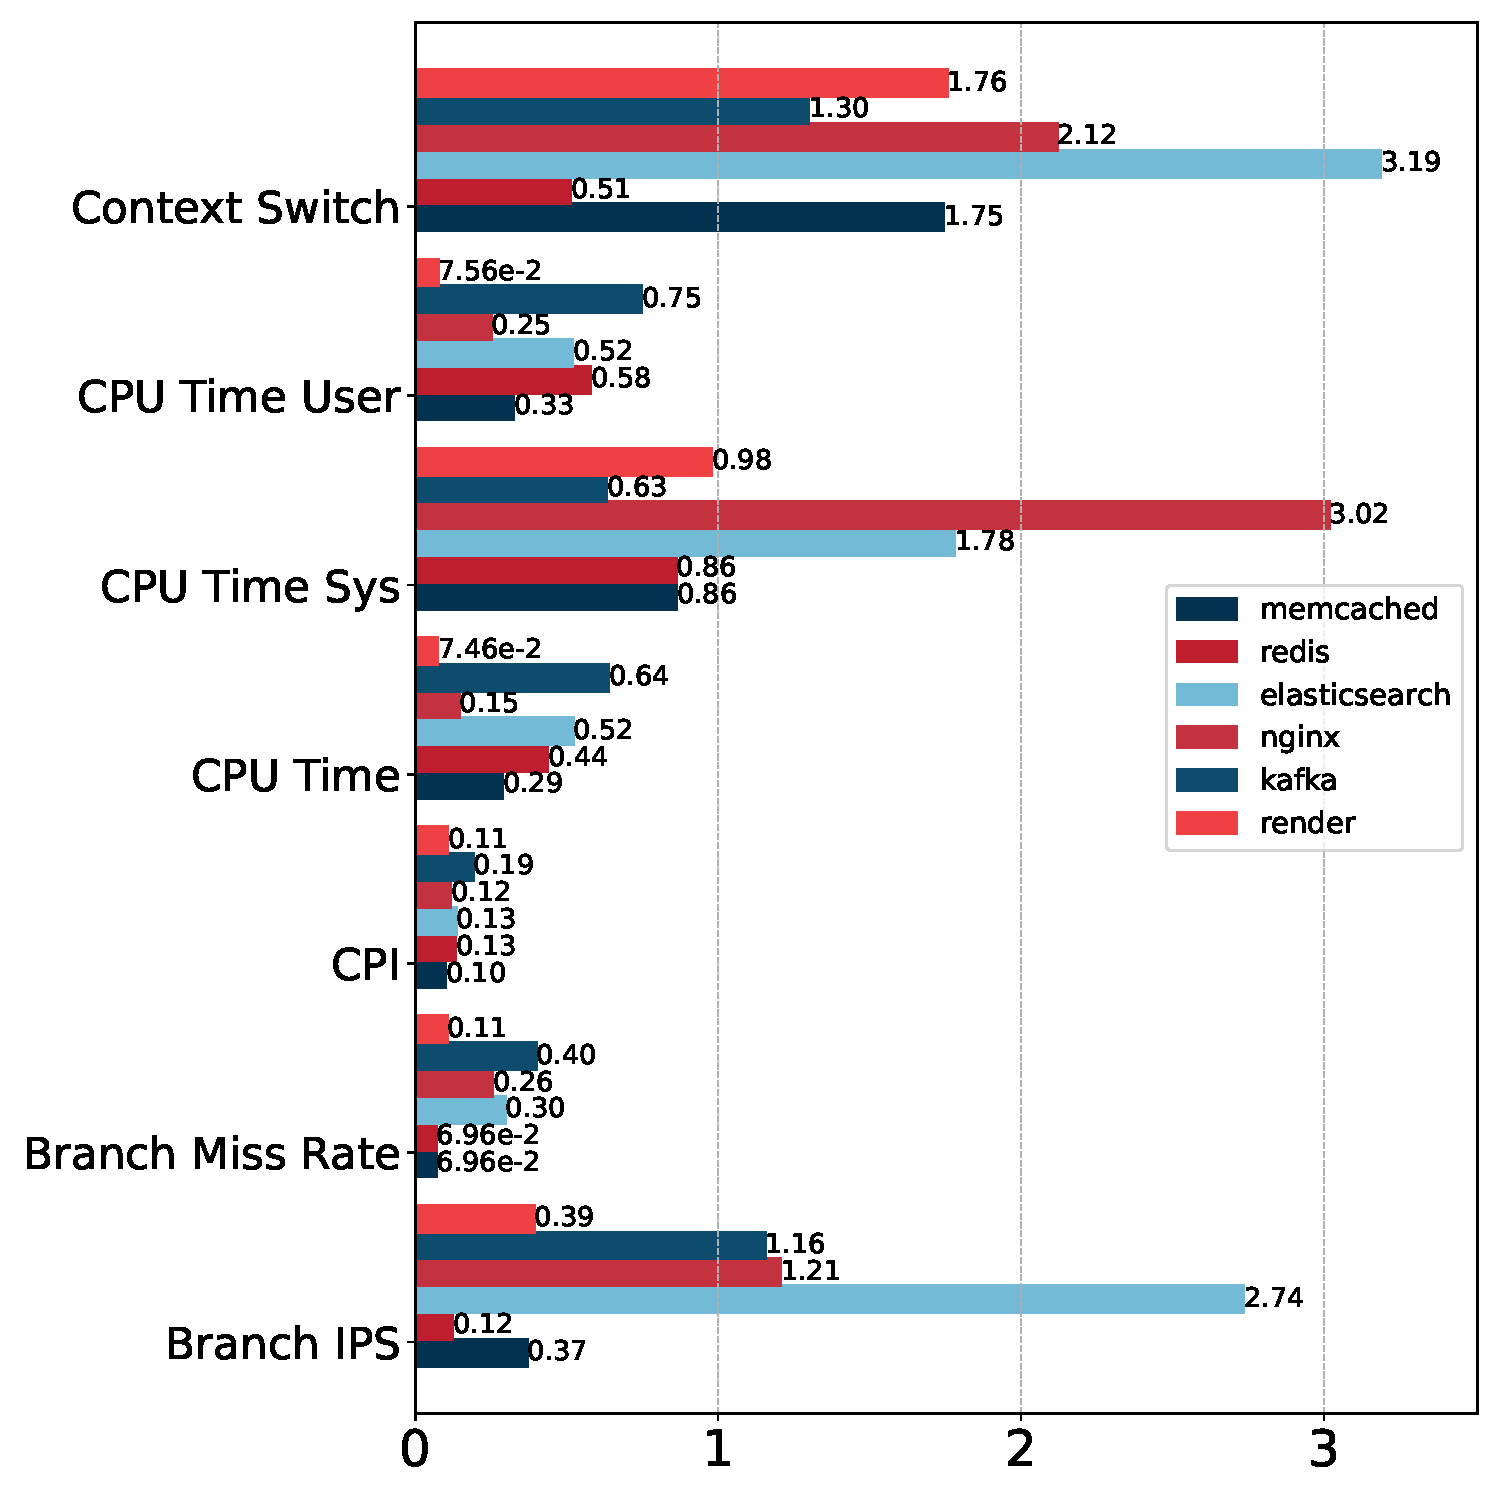
\includegraphics[width=\textwidth]{cof_cpu}
      \caption{CPU资源指标}
      \label{fig:cof_cpu}
    \end{subfigure}
    \begin{subfigure}[b]{0.49\textwidth}
        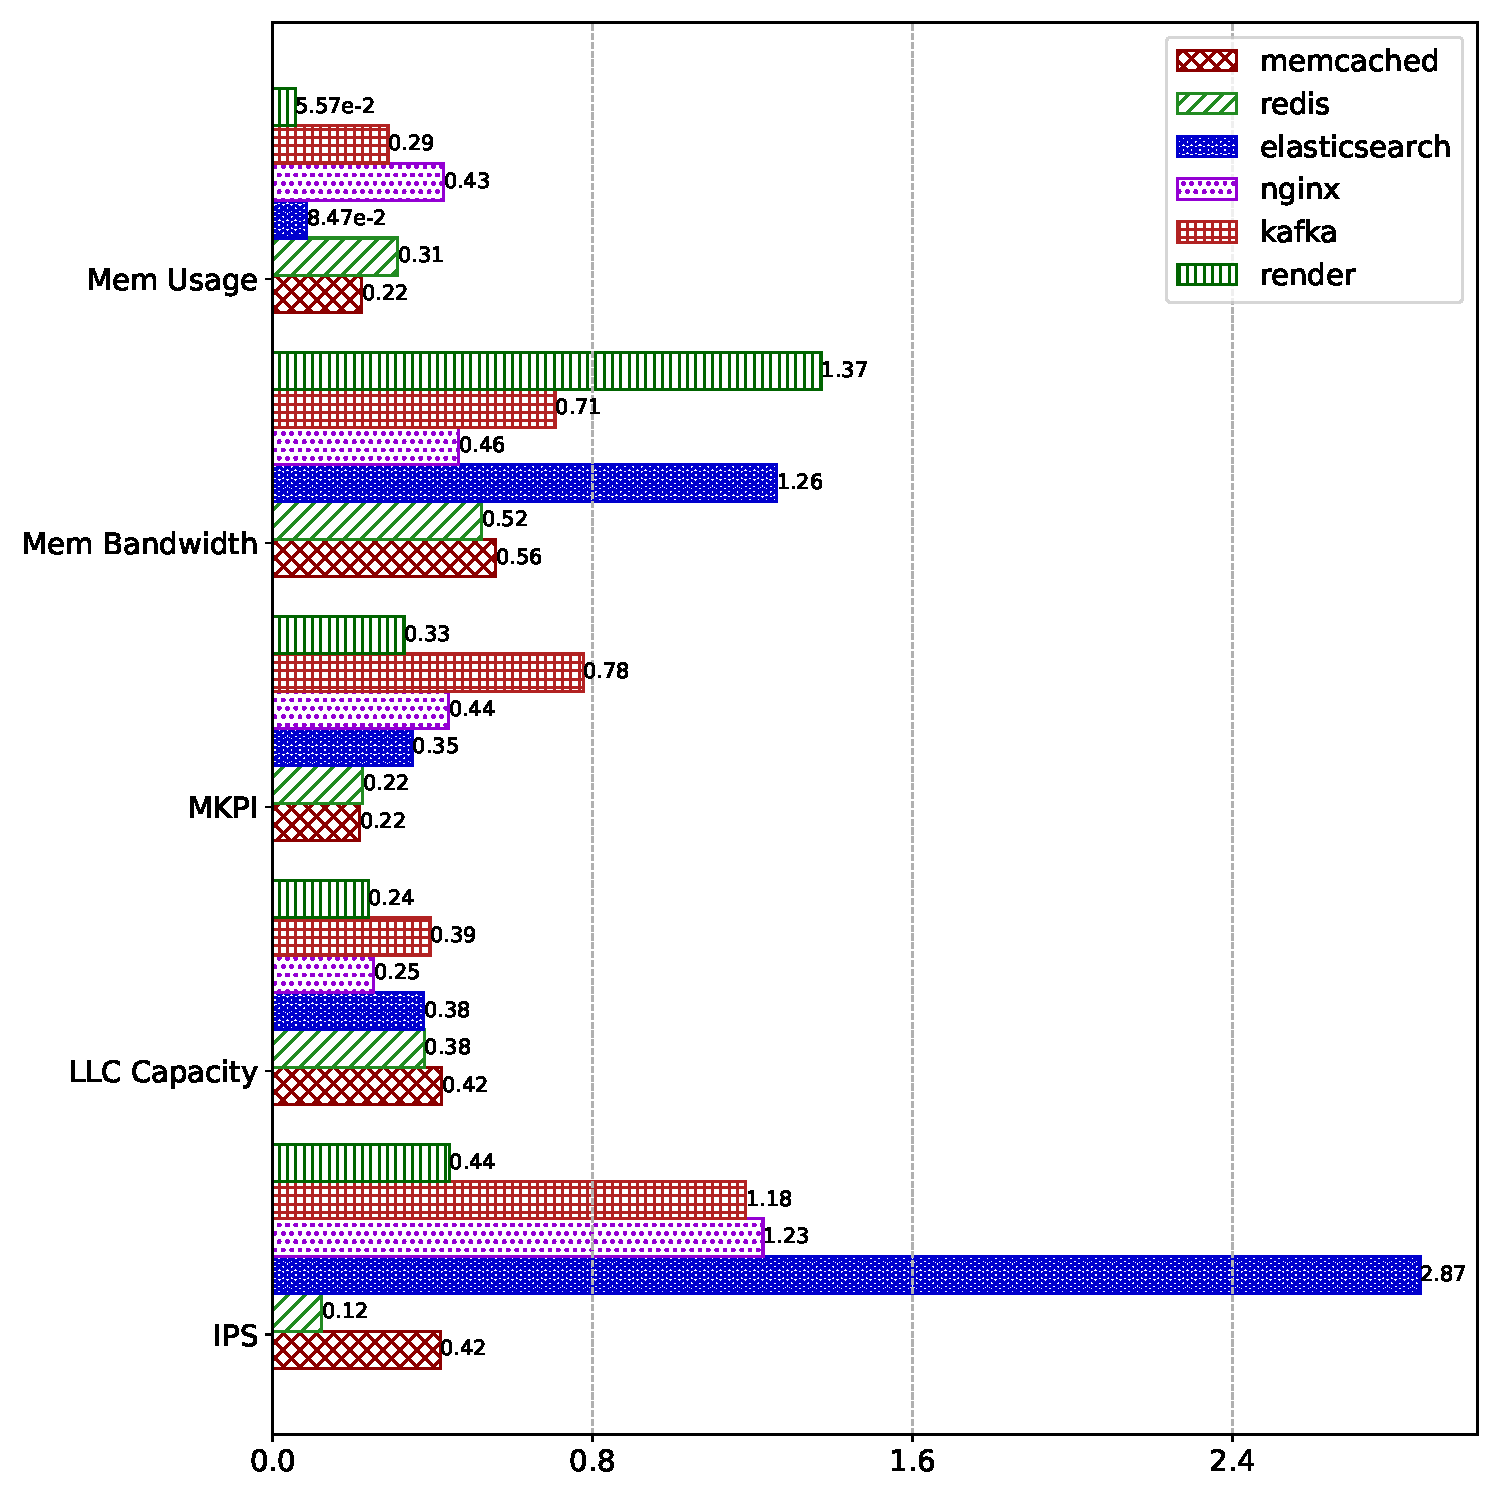
\includegraphics[width=\textwidth]{cof_mem}
        \caption{Cache、内存资源指标}
        \label{fig:cof_mem}
    \end{subfigure}
    \begin{subfigure}[b]{0.49\textwidth}
        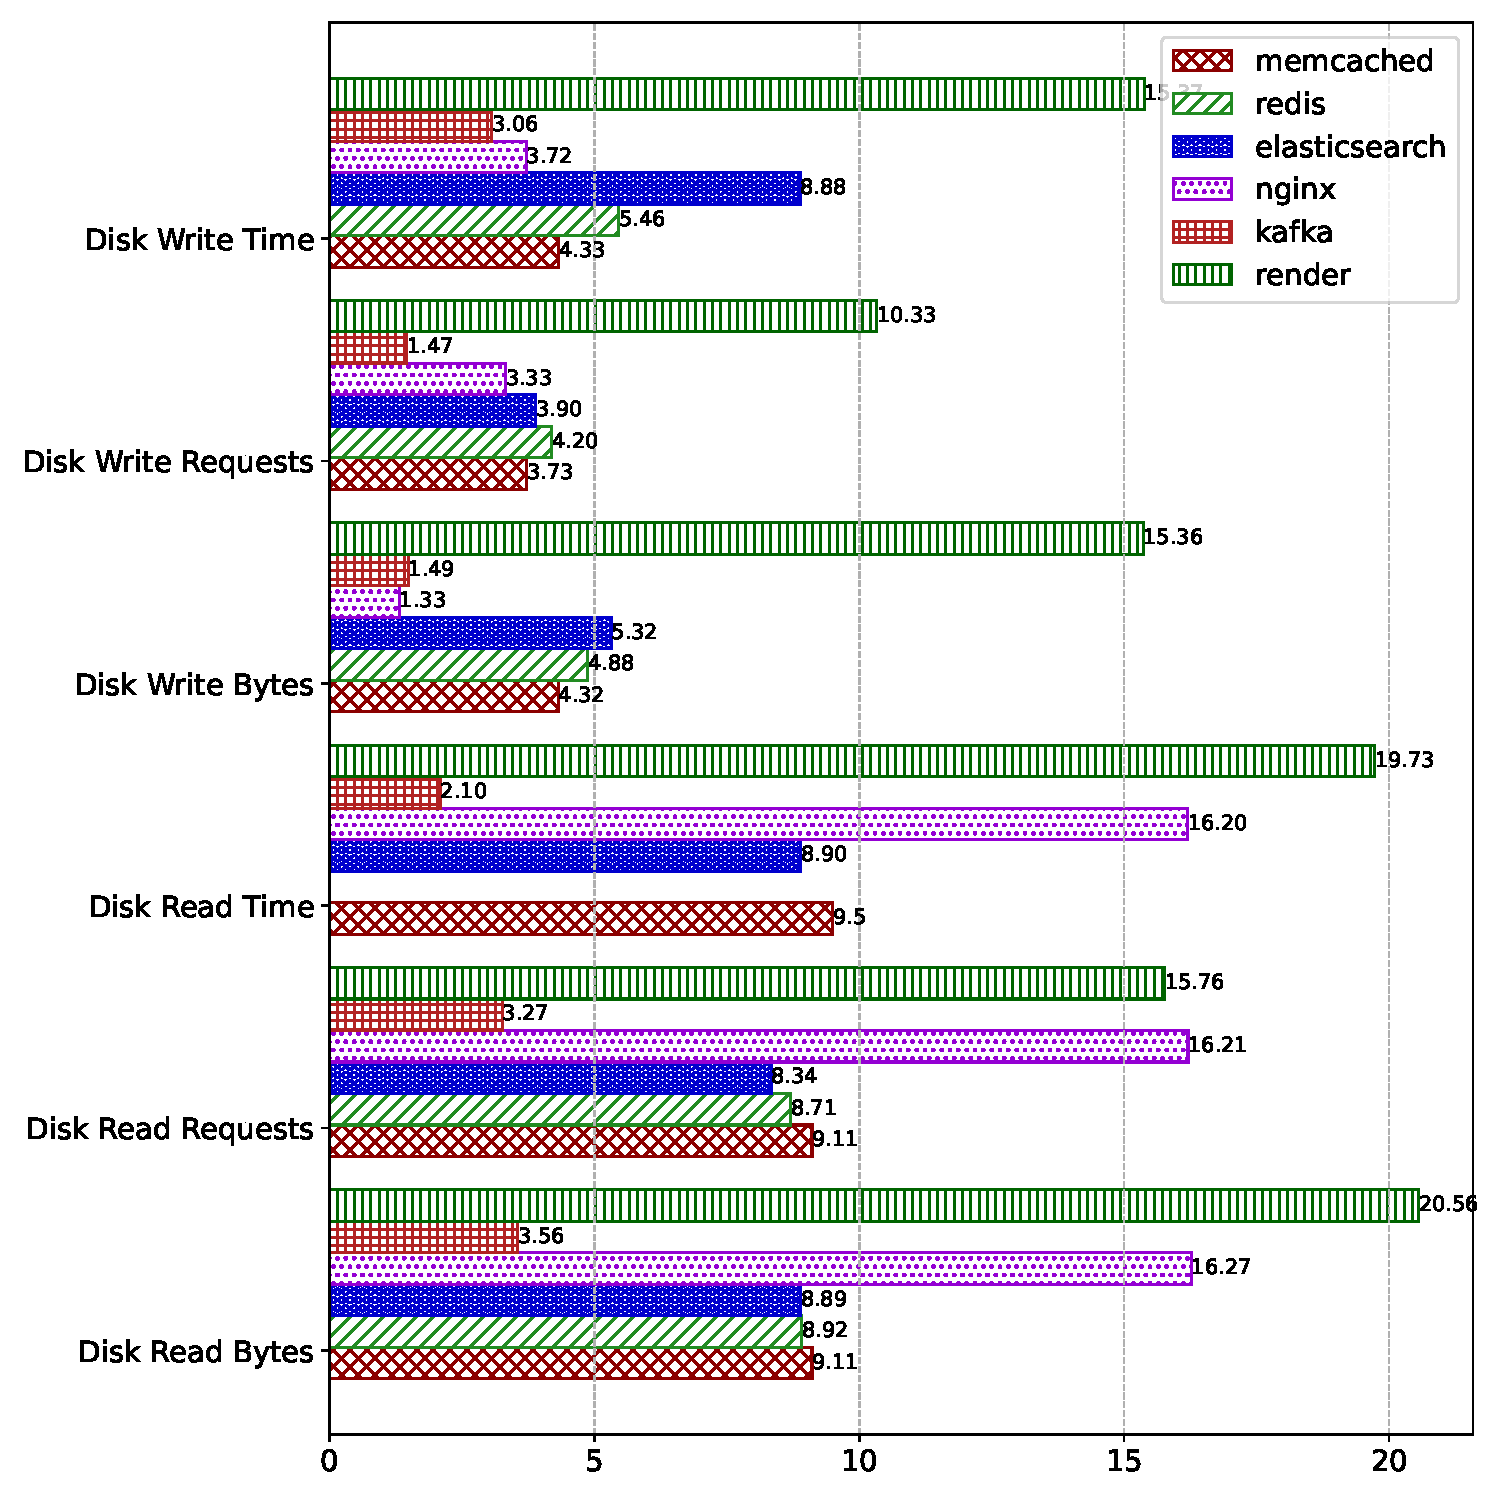
\includegraphics[width=\textwidth]{cof_io}
        \caption{IO资源指标}
        \label{fig:cof_mem}
    \end{subfigure}
    \begin{subfigure}[b]{0.49\textwidth}
        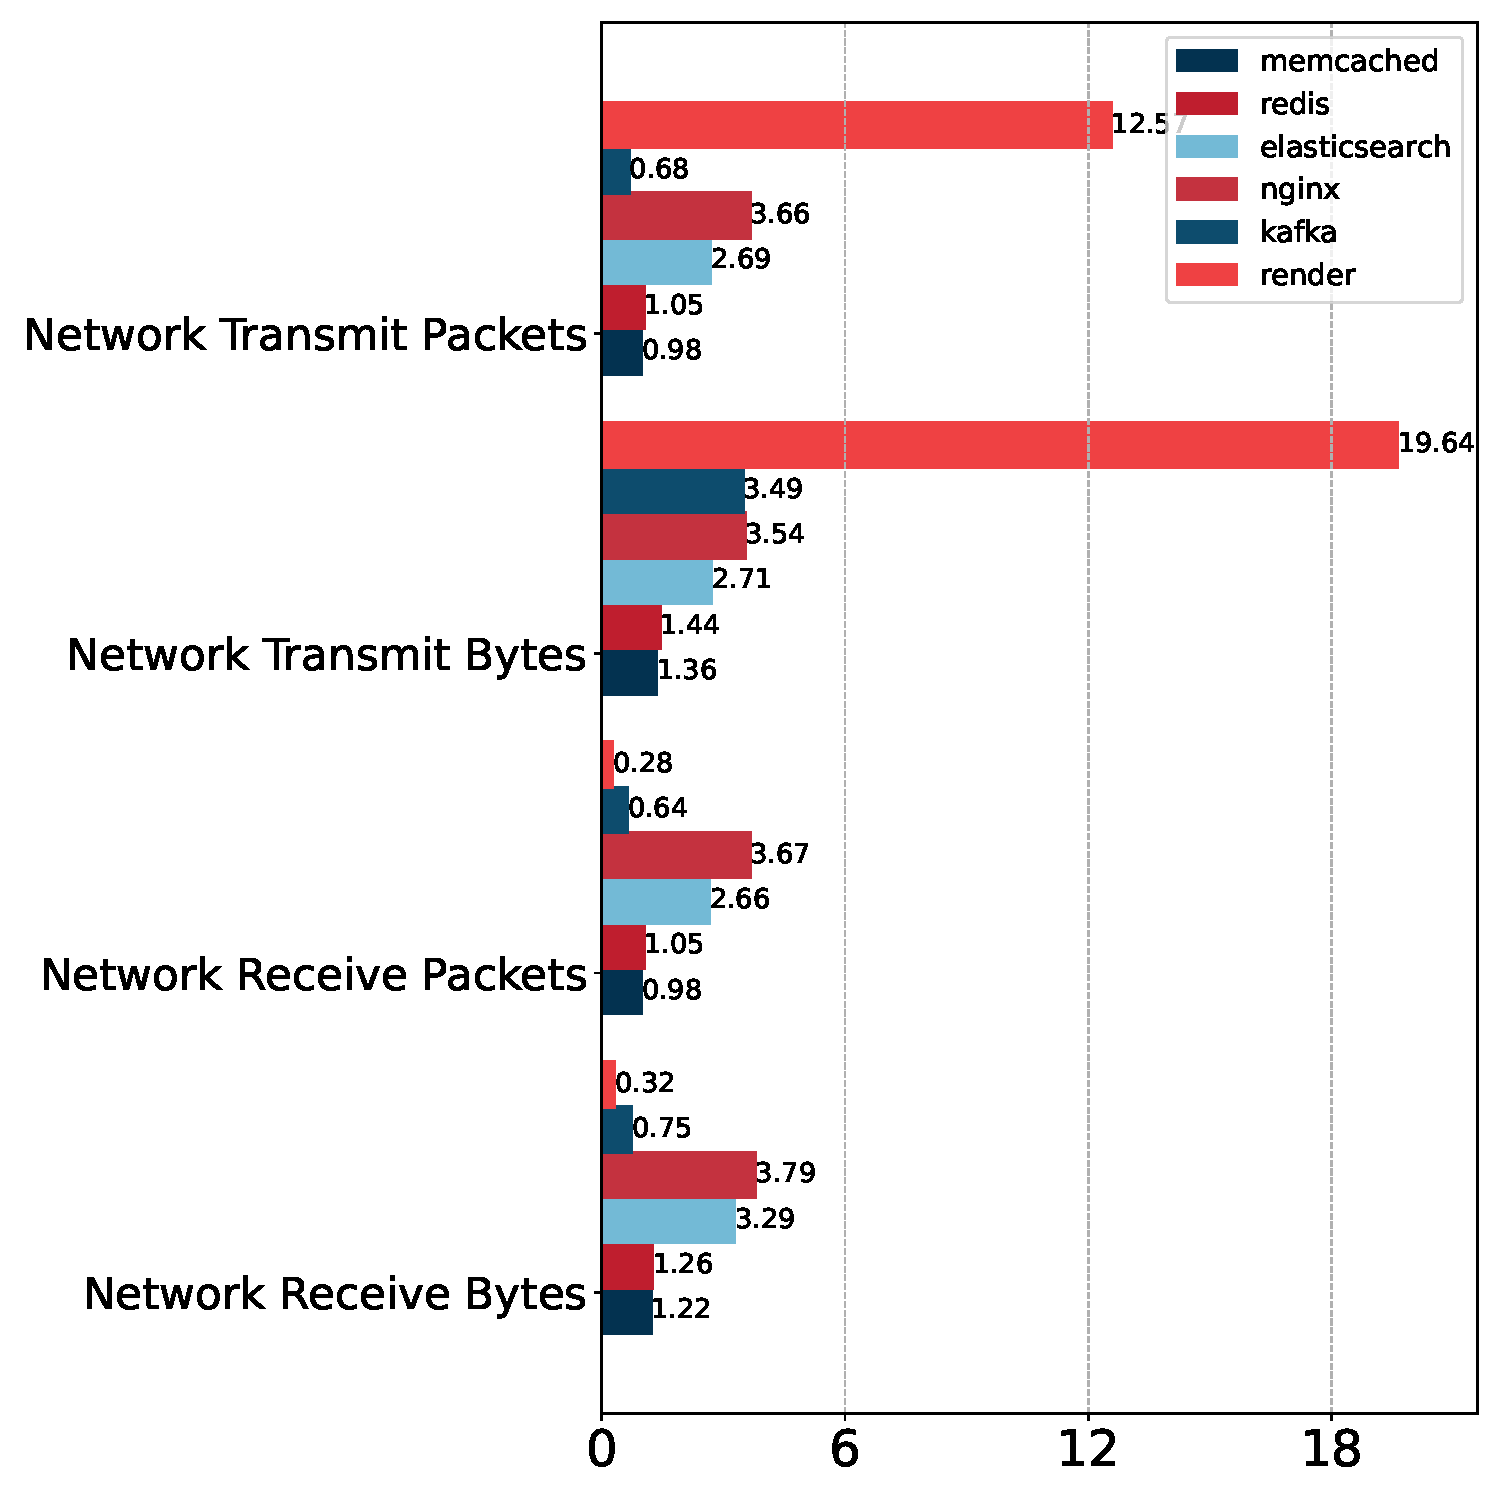
\includegraphics[width=\textwidth]{cof_network}
        \caption{网络资源指标}
        \label{fig:cof_mem}
    \end{subfigure}
\bicaption{\quad 总资源变异系数}{\quad Coefficient of Variation of Total Resources}
\label{fig:resource_affinity}
\end{figure}

从整体上看,Block I/O与Network I/O两类指标在不同应用之间呈现出较大的差异,相同指标在不同应用中的极大值与极小值差异可达$10^4$--$10^5$倍,而其余指标的差异通常不会超过20倍,这就导致图中一部分应用I/O相关指标非常高,而另一部分应用的相同指标则始终为一个较低的值。而在其他指标上则没有体现明显的差异度,这有如下两方面原因,首先,对于"利用率"类型的指标,这些指标存在明确的上下界,同时数值上的差异度难以直接体现,如对于CPU利用率,80\%与90\%利用率仅有约12\%的数值差异,但计算空闲CPU占比,则前者是后者的200\%,对于这些指标不能简单地使用差异度度量。其次,一些与硬件相关的指标波动不明显,如CPI,其波动通常受到流水线周期、指令阻塞和回退的数量等因素影响,在优化较好的现代处理器平台上,通常只会在一个较小的范围内波动。

\begin{figure}[H]
    \centering
    \begin{subfigure}[b]{0.9\textwidth}
      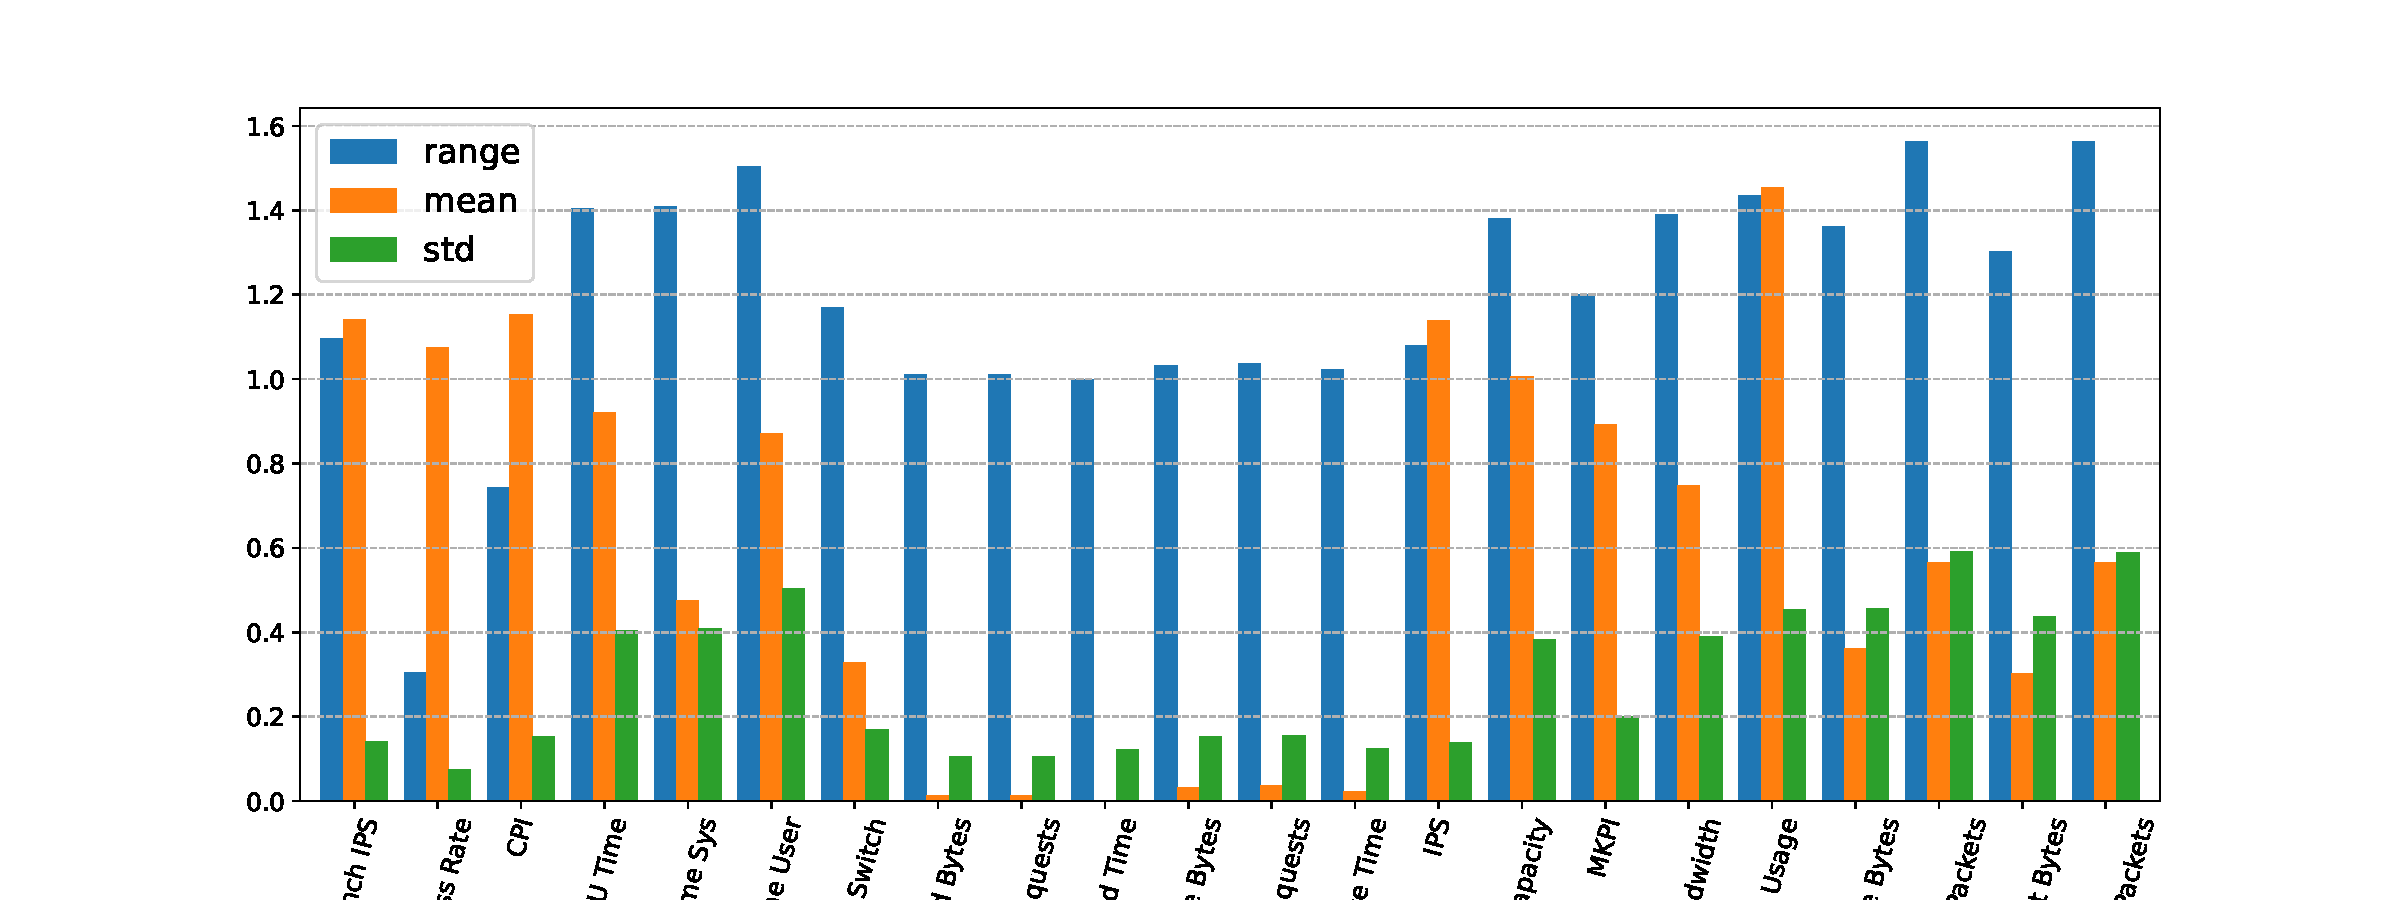
\includegraphics[width=\textwidth]{profile_redis}
      \caption{Redis资源使用}
      \label{fig:profile_redis}
    \end{subfigure}
    \begin{subfigure}[b]{0.9\textwidth}
        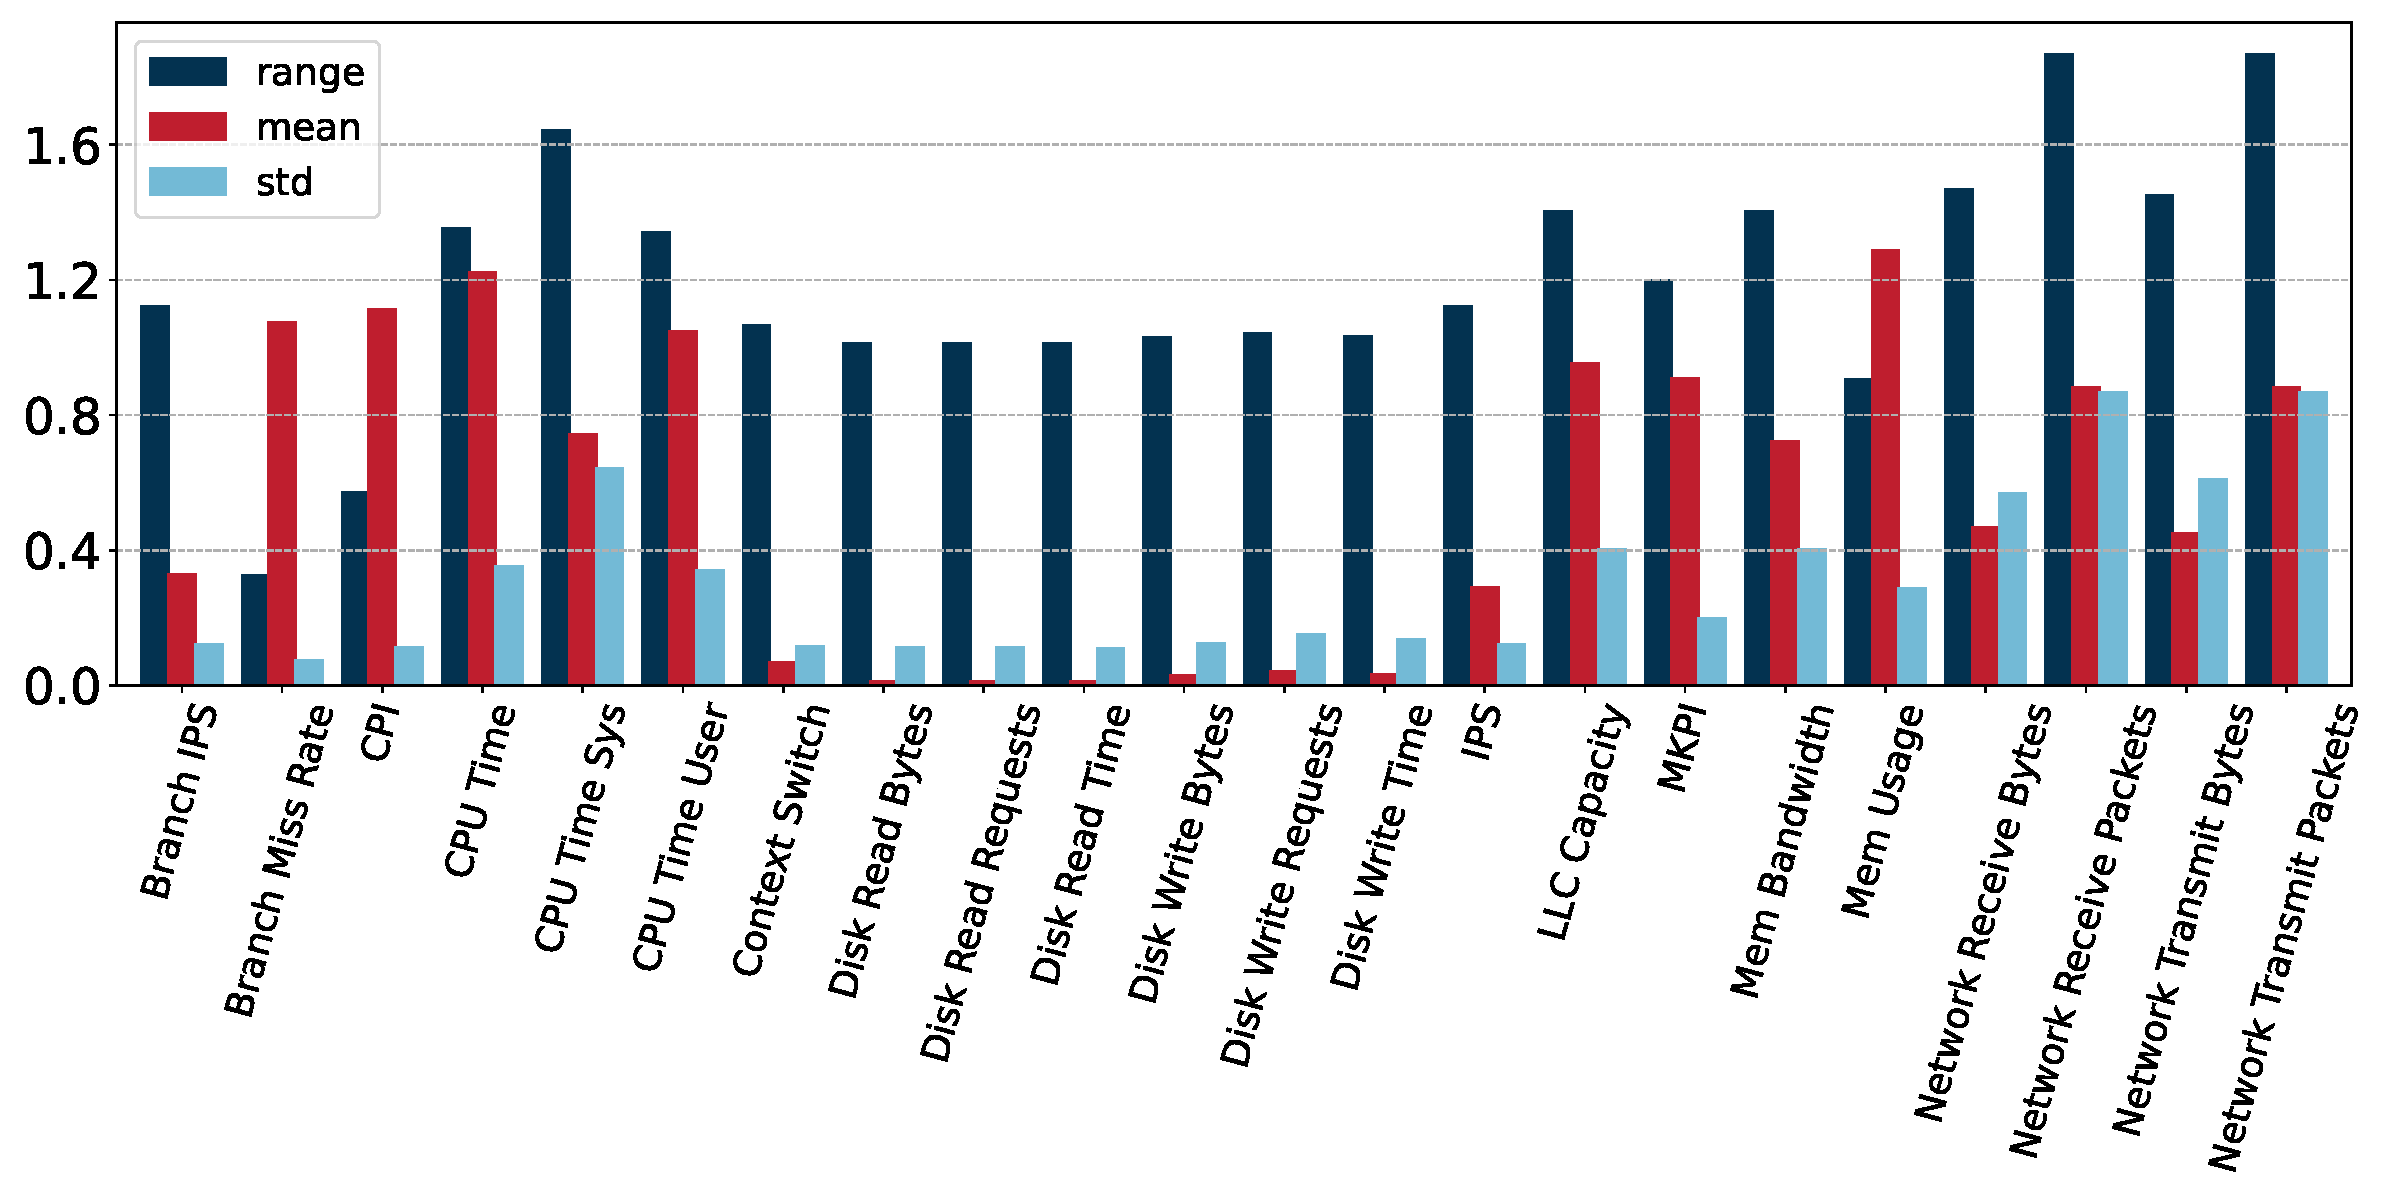
\includegraphics[width=\textwidth]{profile_memcached}
        \caption{Memcached资源使用}
        \label{fig:profile_memcached}
    \end{subfigure}
\bicaption{\quad Redis与Memcached资源使用情况}{\quad Resource Usage of Redis and Memcached}
\label{fig:resource_affinity_0}
\end{figure}

具体到应用的差异性如图~\ref{fig:resource_affinity_0}所示,不同应用对于主要的5种系统资源的需求呈现处较大的差异:

\begin{enumerate}
    \item CPU资源:应用的运行都需要CPU资源, 而不同应用对于CPU资源的使用上存在差异。Kafka运行时需要较多的CPU资源,体现在较高的IPS指标上。Redis、Memcached同样对于CPU资源有较高需求,从较多的平均CPU时间片占用能够看出,但不同之处在于,Redis、Memcached对于CPU资源的使用与请求强相关,在请求量较低时,由于频繁的睡眠与唤醒,此时不仅CPU资源需求少,同时CPI也较高,而当请求量足够多时,由于都基于epoll实现,因此密集的请求使得两者总是能够保持CPU的占用,而相较于Redis,Memcached在默认配置下更能够利用多核优势。Render应用同样需要较多的CPU资源,但与上述应用不同的是,Render在CPU资源使用上相当稳定,这一特点反映在较低的Branch IPS及Context Switch指标上。
    \item Cache资源:末级缓存资源与内存访问强相关,分析不同应用的LLC相关指标,可以将应用按访存局部性进行划分,其中Niginx属于局部性较好的应用,其在运行过程中LLC使用率波动不明显,并且LLC Miss数量较少。而对于Redis、Memcached这类键值存储型应用,局部性则与工作负载相关,在随机负载下局部性表现较差,而在模拟负载下局部性则相对较好。
    \item Memory资源:内存资源区分带宽与使用量。典型应用中,Nginx在模拟负载下对内存带宽的需求较高,这点与其在Cache资源需求上的表现一致,而其余应用则采用间歇与分批的内存读取,因此不会占用过多的内存带宽。而在内存使用量上,典型应用的内存占用除自身所需外,都与工作负载相关,而在华为云的默认负载下,各个应用都会占用一定量的内存而并没有特别的规律性。
    \item Network资源:在网络资源上,不同的应用使用需求差异很大,其中Redis、Memcached、Kafka表现出极高的网络需求,事实上这些应用都是服务型应用或自身就是网络消息中间件。而Elasticsearch、Render等在网络资源的需求上则相对较少,其中Elasticsearch并非不使用网络,而因为工作负载中并没有长时间且持续性的请求,Render则因为是离线应用,因此几乎不会使用到网络资源。
    \item I/O资源:在I/O资源上,不同应用的使用需求差异同样十分大。其中Elasticsearch、Kafka和Mysql由于涉及到存储内容的持久化,因此会大量地使用I/O资源。而类似Redis等应用,虽然存在数据持久化的配置,但实际运行中持久化频率较低,因此通常只会有周期性的少量I/O资源占用。
\end{enumerate}

\begin{figure}[H]
    \centering
    \begin{subfigure}[b]{0.9\textwidth}
      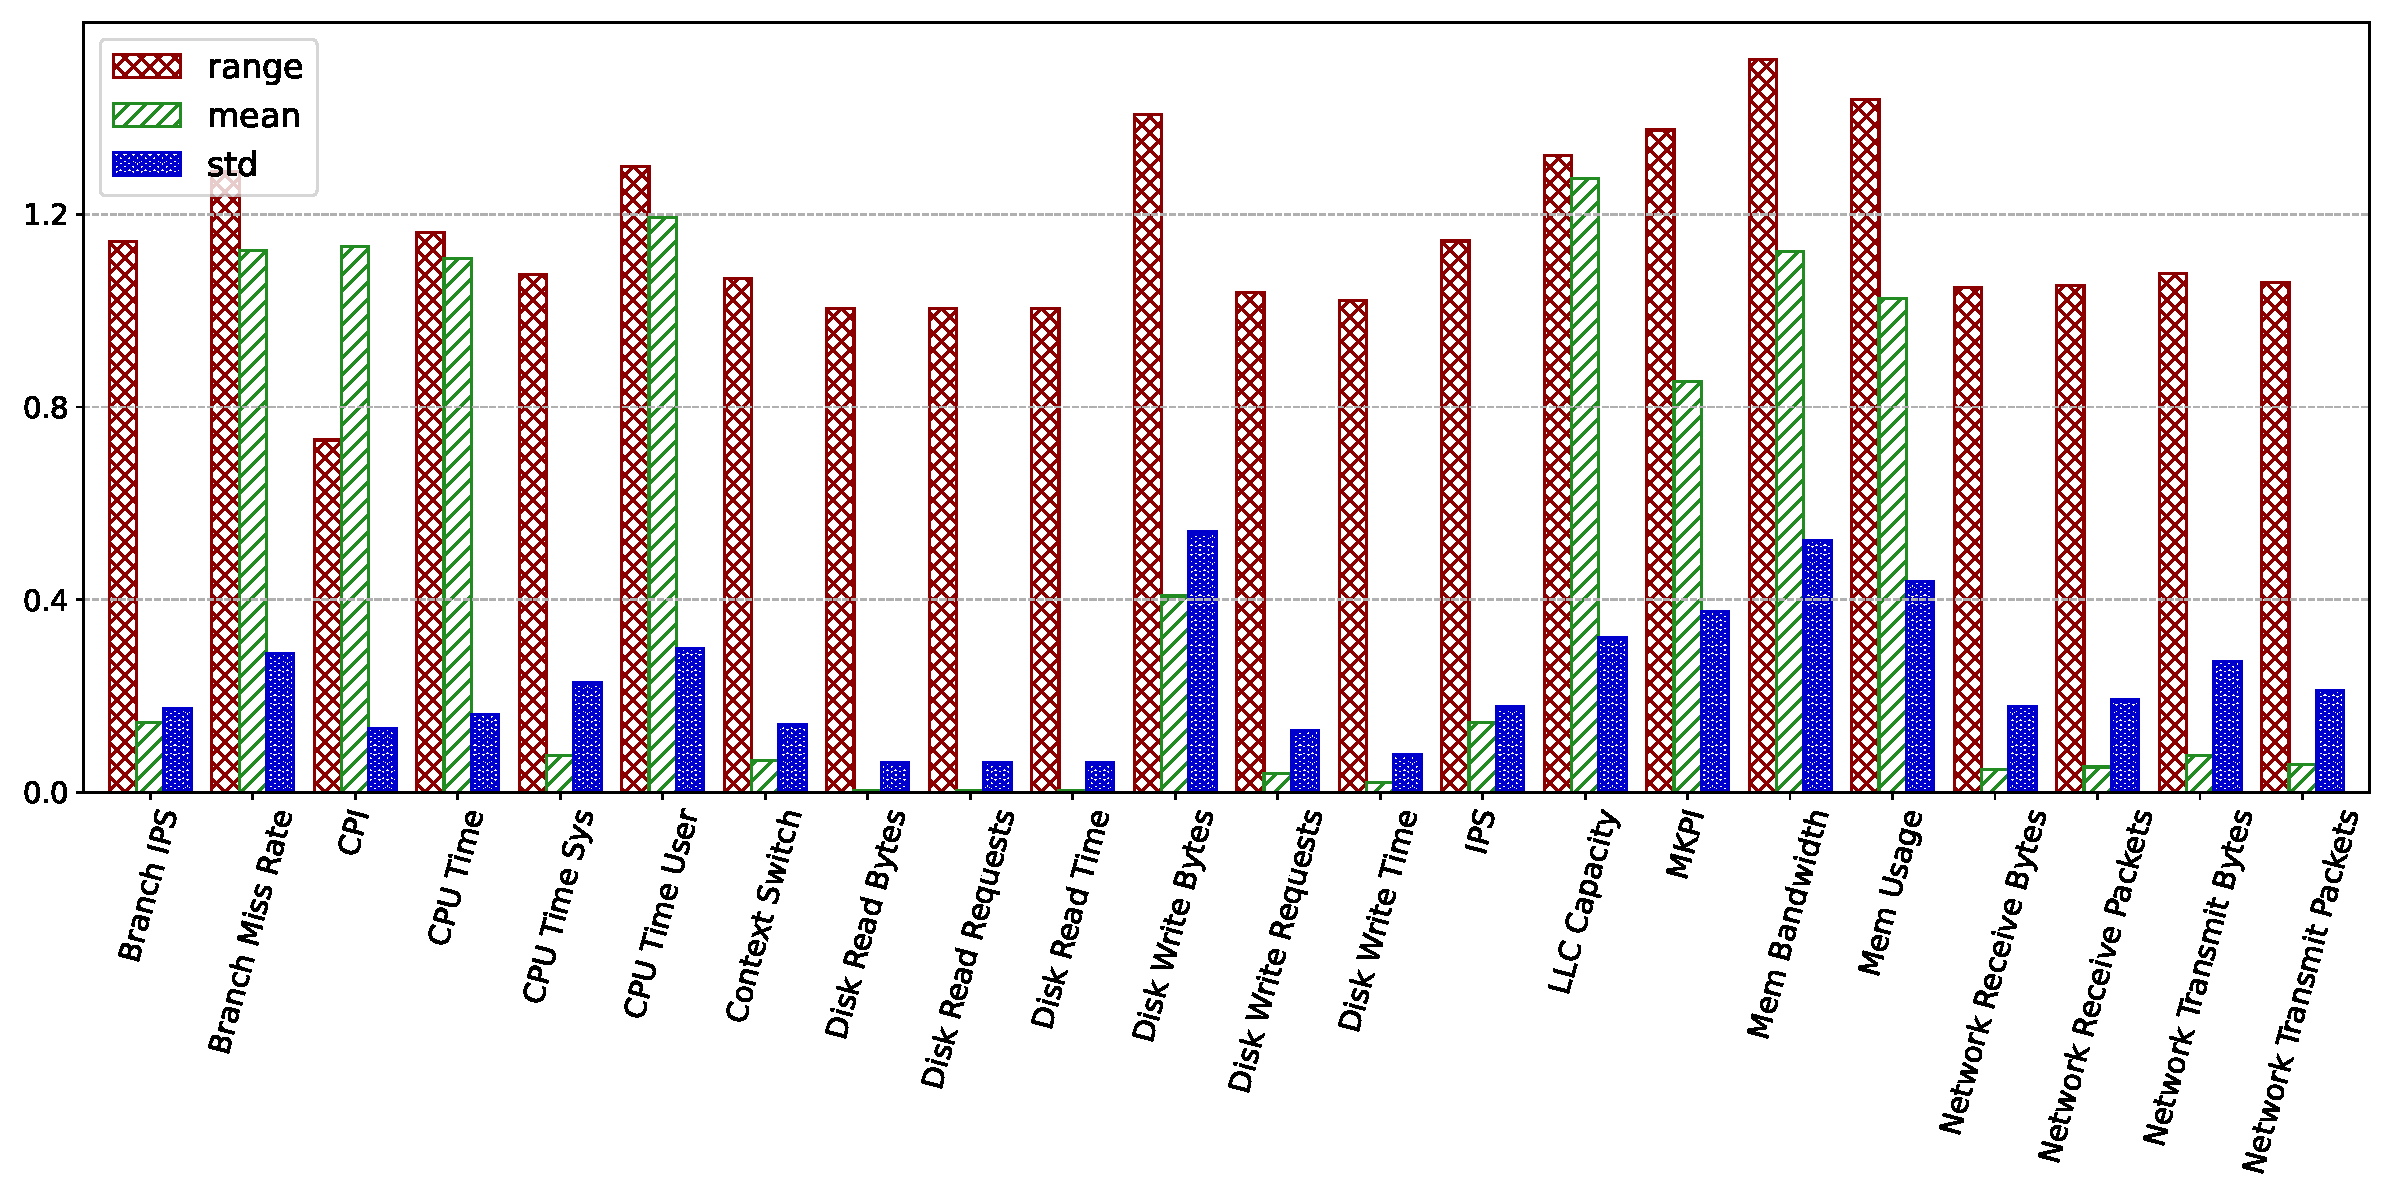
\includegraphics[width=\textwidth]{profile_nginx}
      \caption{Nginx资源使用}
      \label{fig:profile_nginx}
    \end{subfigure}
    \begin{subfigure}[b]{0.9\textwidth}
        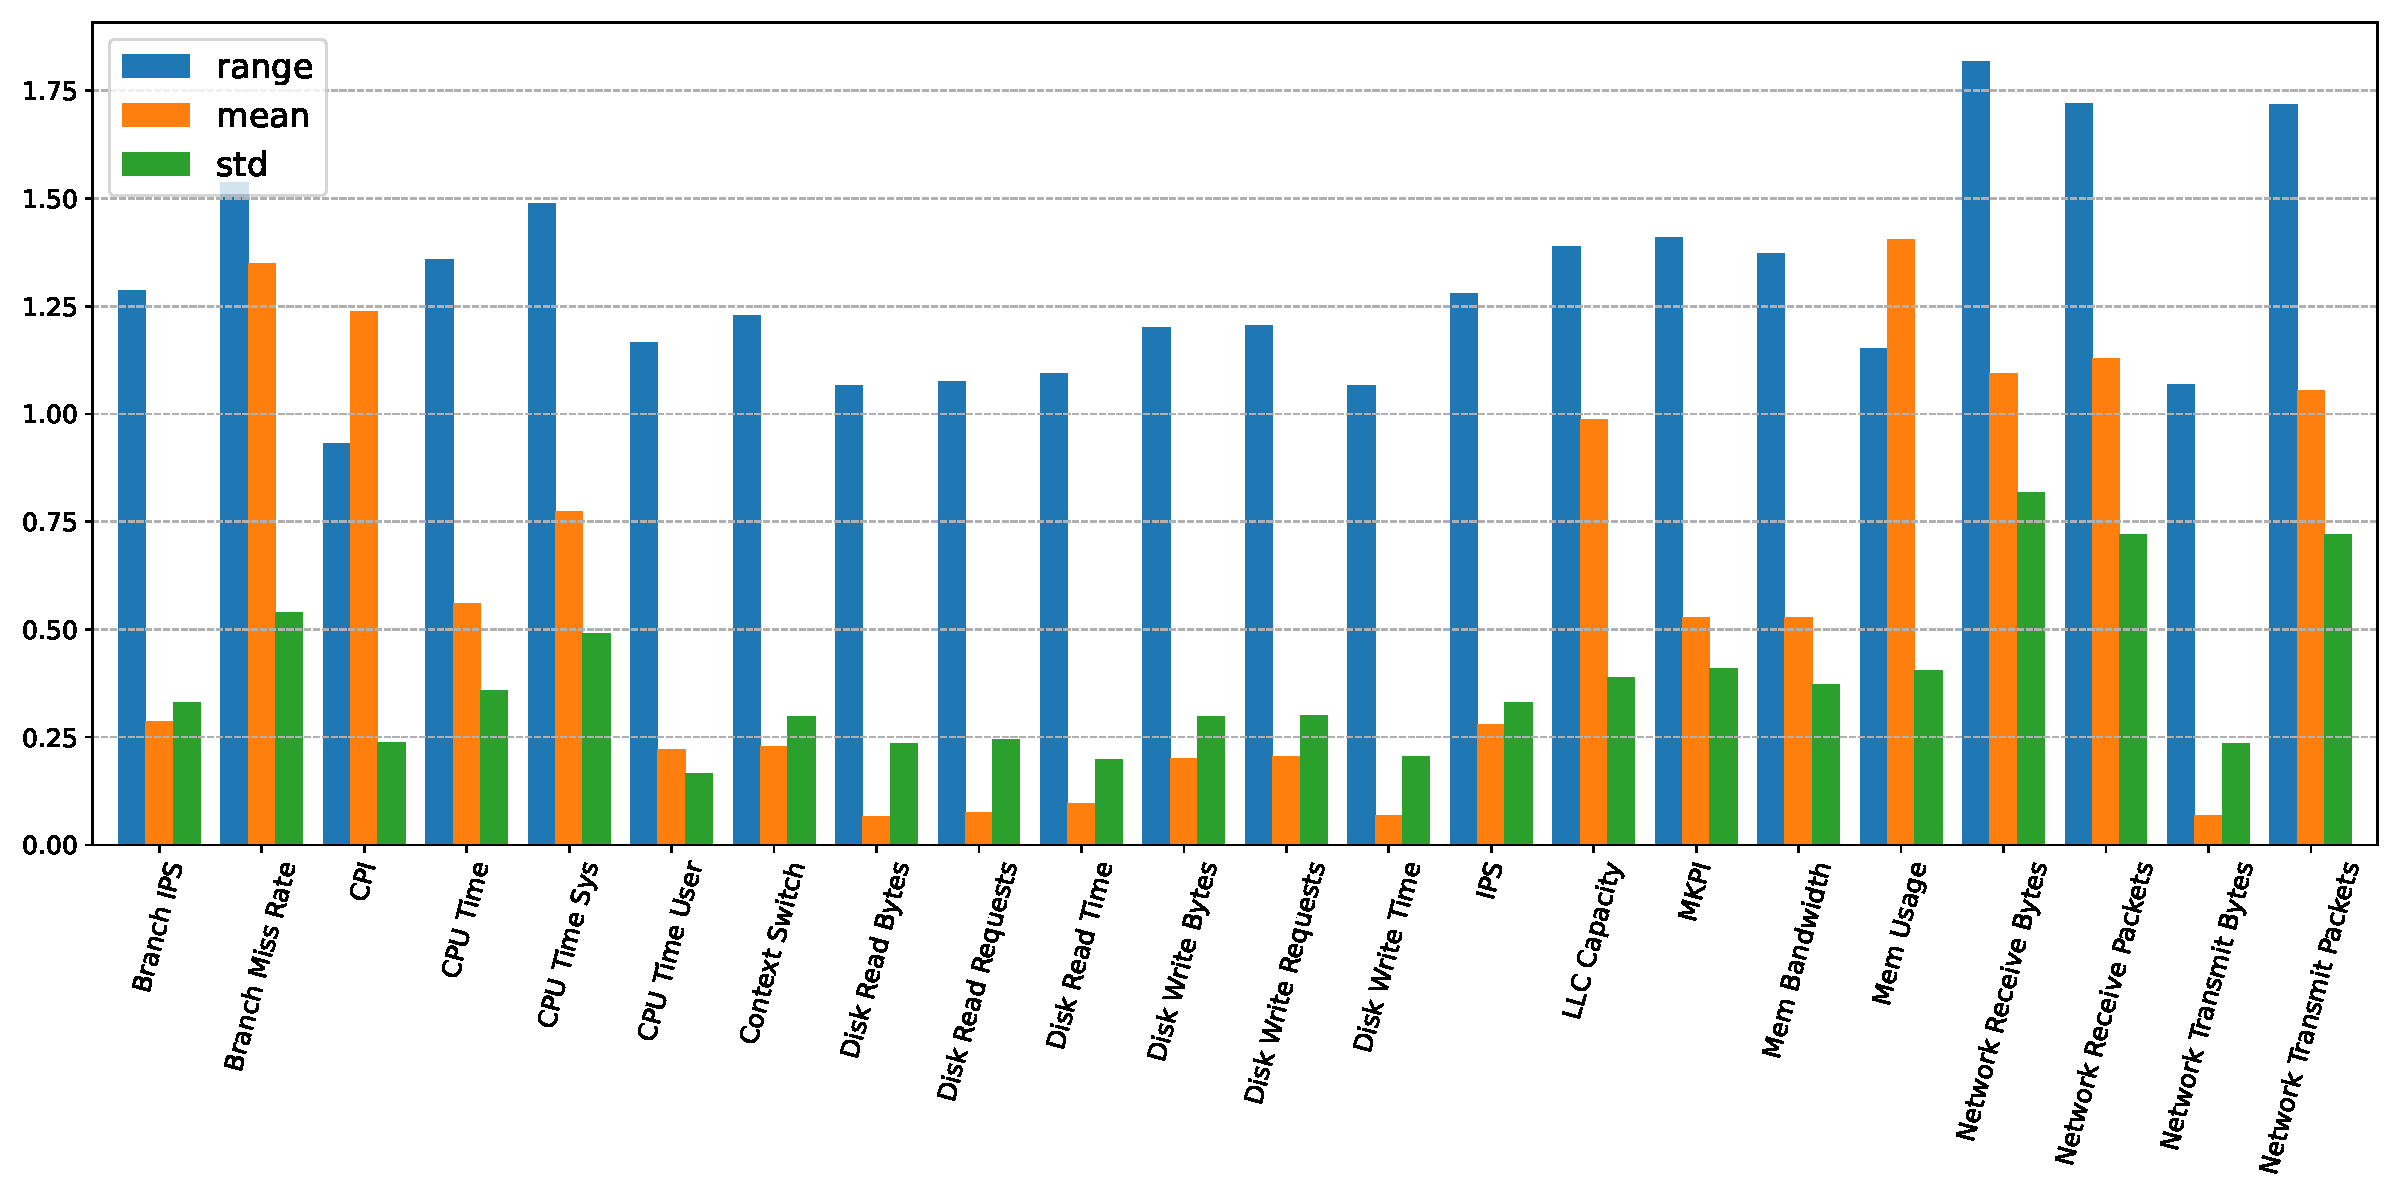
\includegraphics[width=\textwidth]{profile_kafka}
        \caption{Kafka资源使用}
        \label{fig:profile_kafka}
    \end{subfigure}
\bicaption{\quad Nginx与Kafka资源使用情况}{\quad Resource Usage of Nginx and Kafka}
\label{fig:resource_affinity_1}
\end{figure}

\begin{figure}[H]
    \centering
    \begin{subfigure}[b]{0.9\textwidth}
      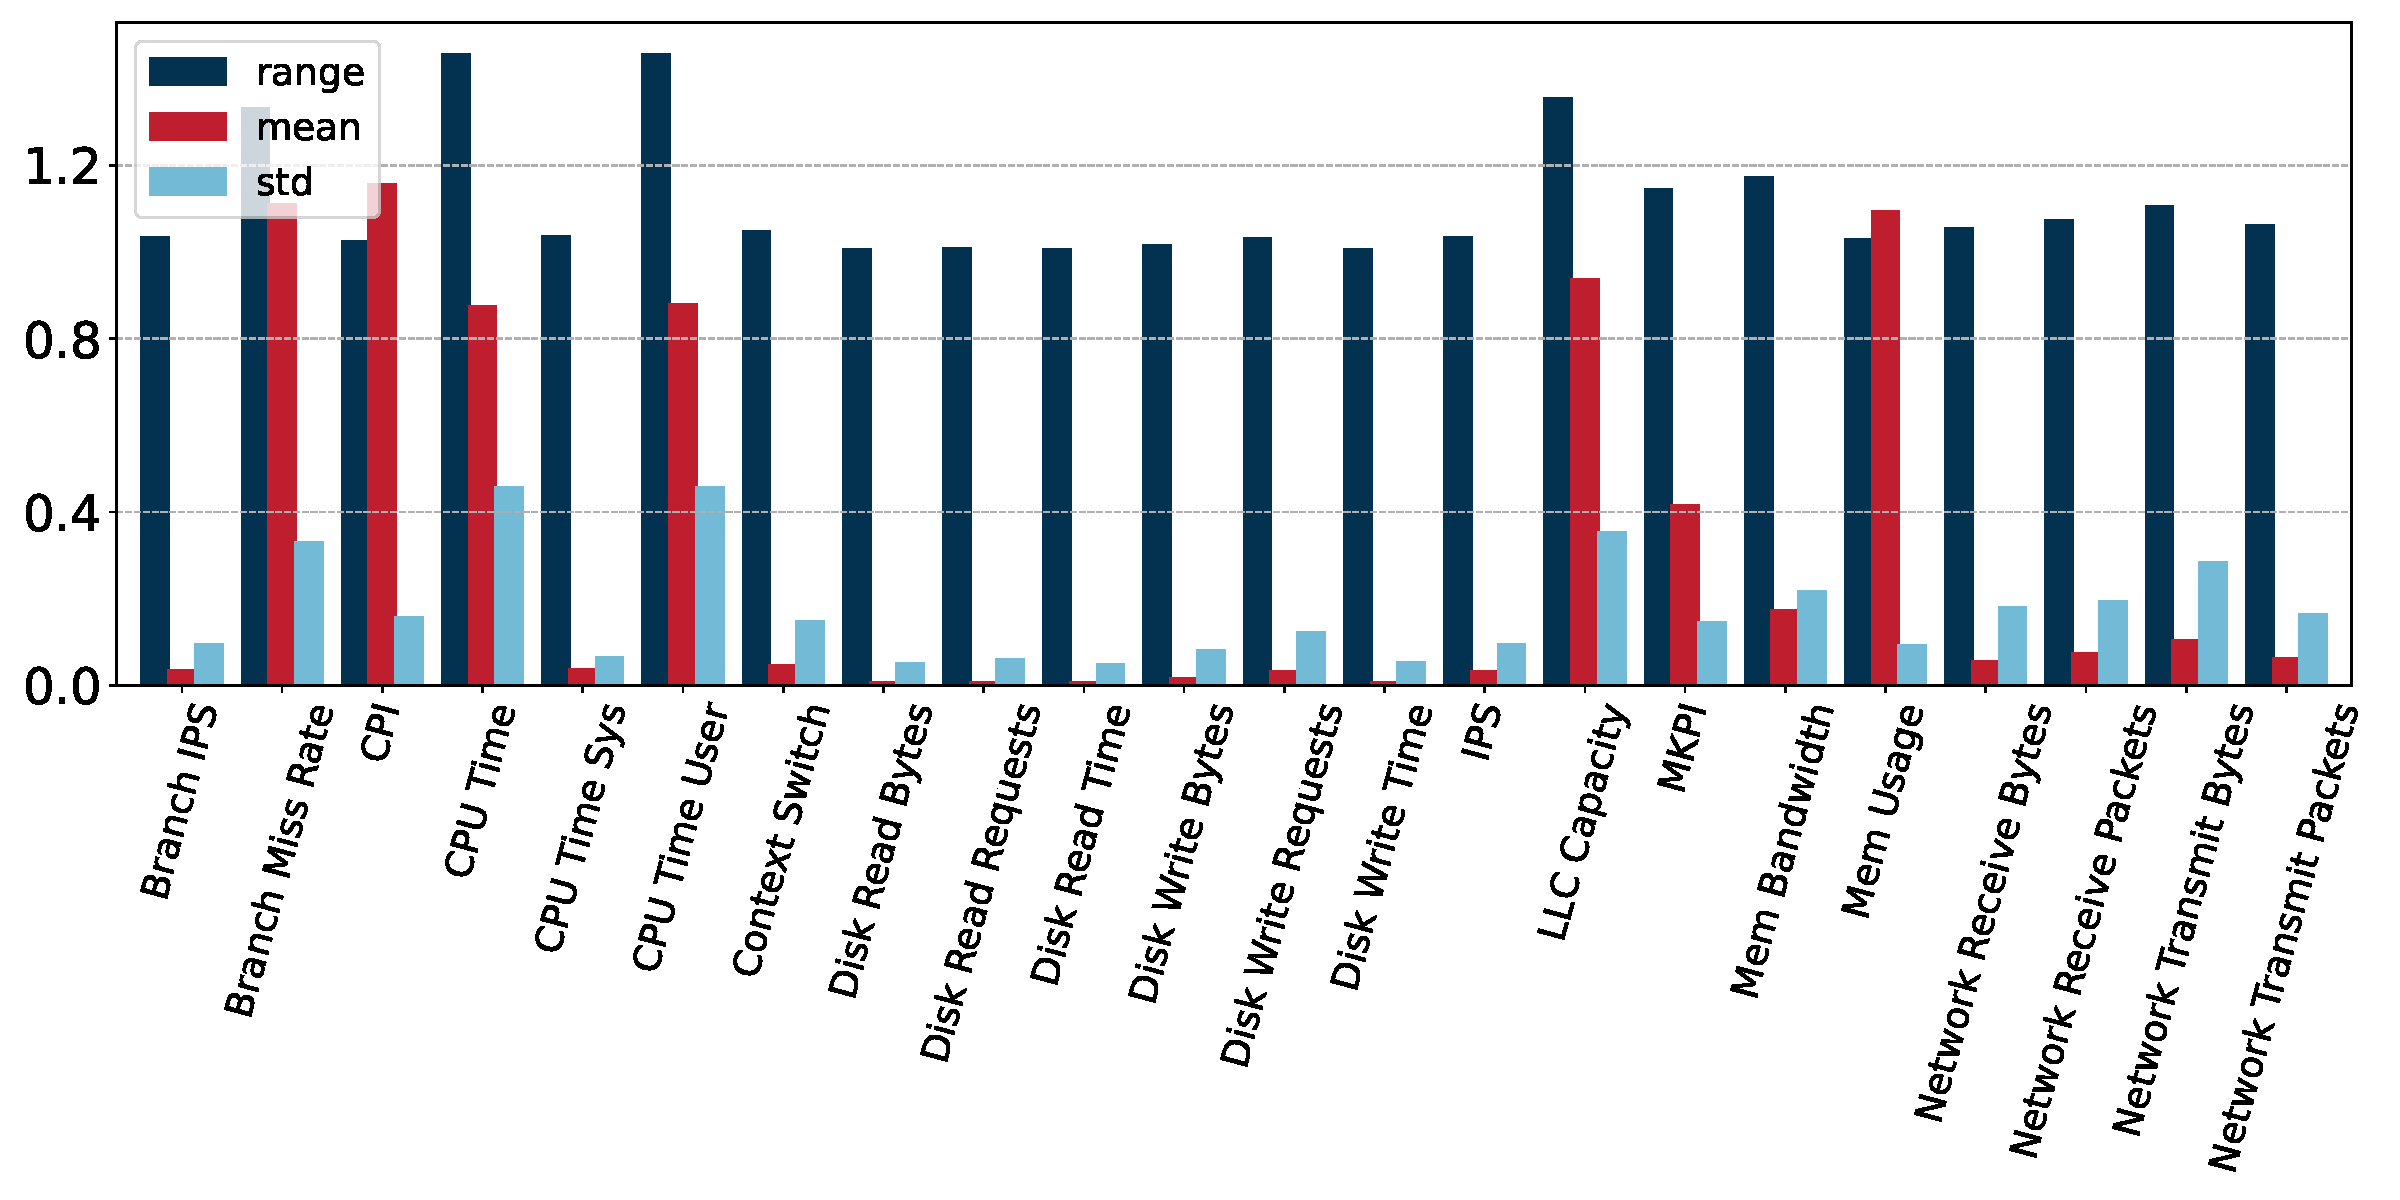
\includegraphics[width=\textwidth]{profile_elasticsearch}
      \caption{Elasticsearch资源使用}
      \label{fig:profile_elasticsearch}
    \end{subfigure}
    \begin{subfigure}[b]{0.9\textwidth}
        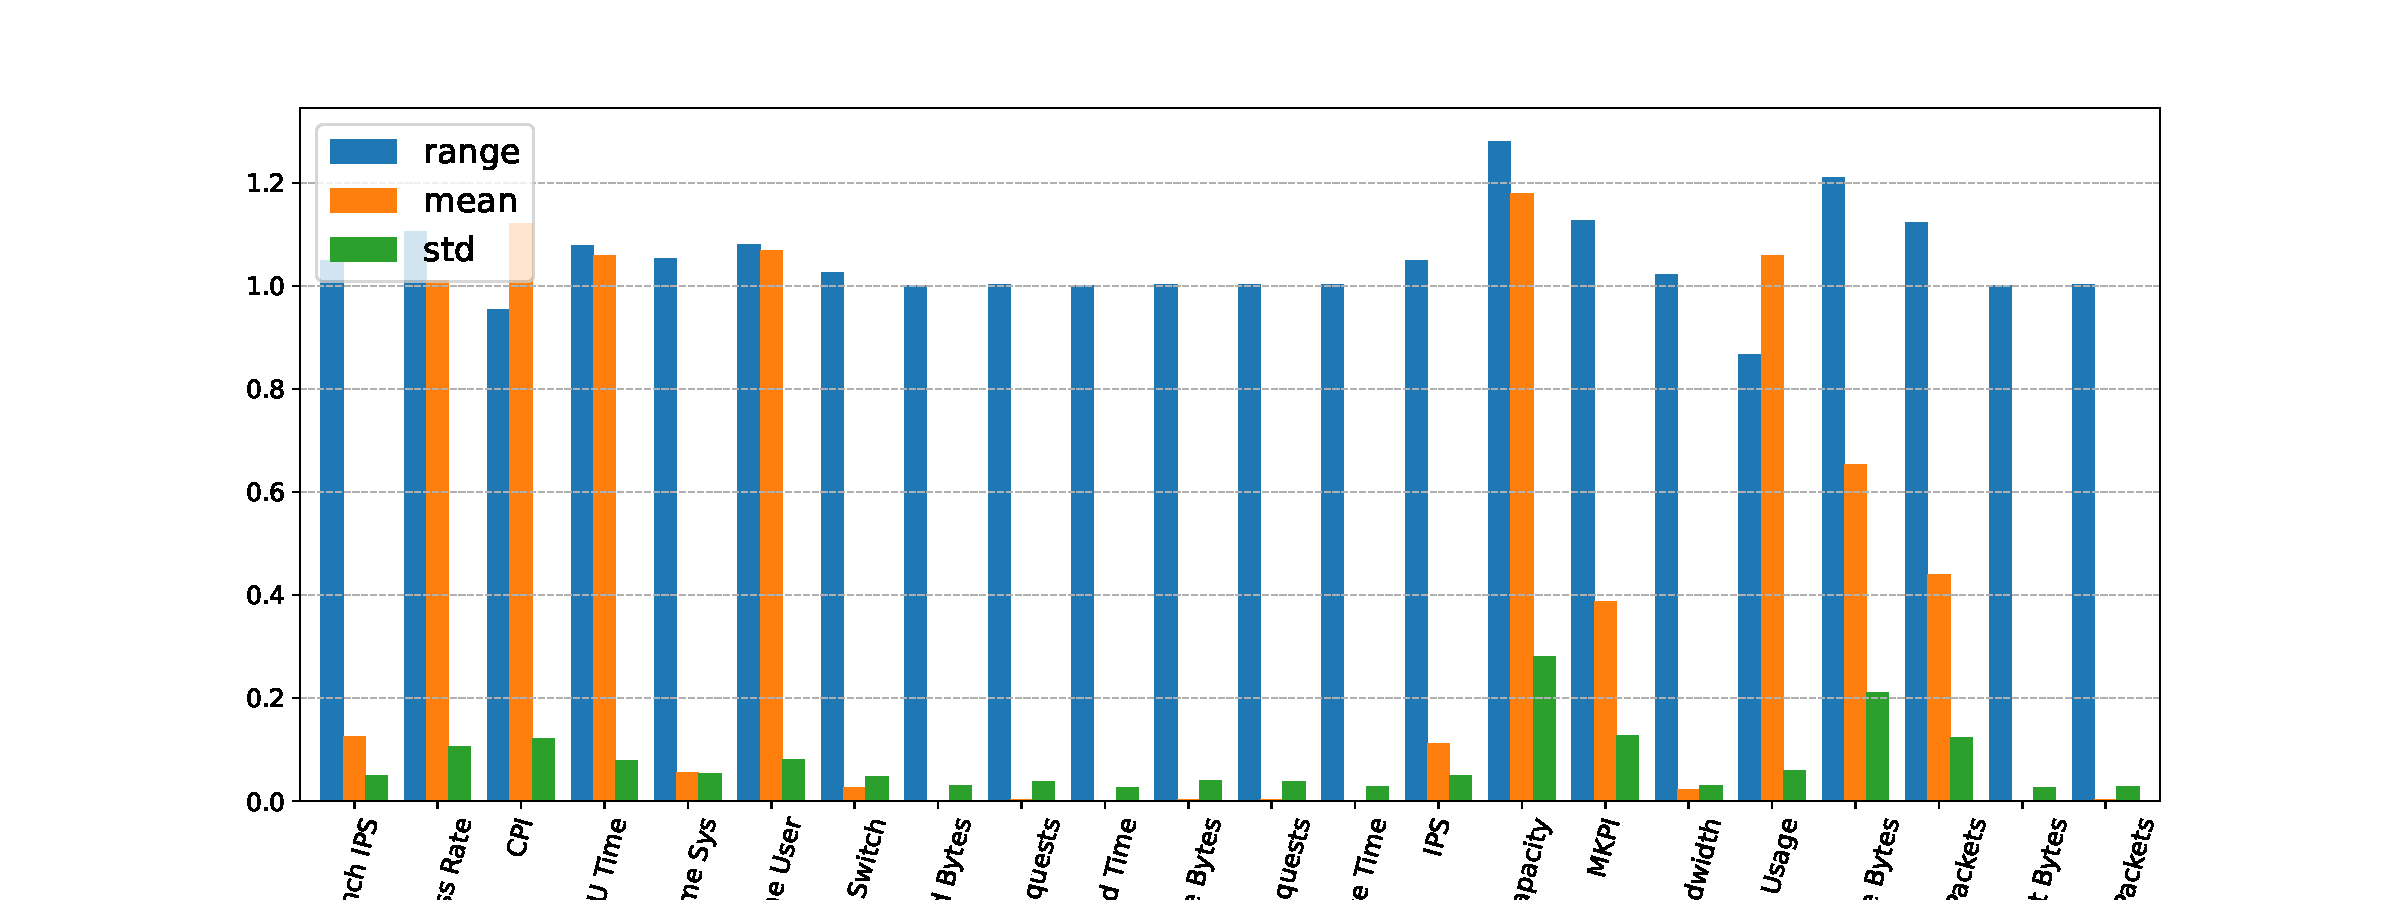
\includegraphics[width=\textwidth]{profile_render}
        \caption{Render资源使用}
        \label{fig:profile_render}
    \end{subfigure}
\bicaption{\quad Elasticsearch与Render资源使用情况}{\quad Resource Usage of Elasticsearch and Render}
\label{fig:resource_affinity_2}
\end{figure}

\section{性能劣化实验设计与分析}

\subsection{干扰实验设计}

% 干扰应用
% - 干扰有效性
% - 噪声控制

性能劣化实验通过增加目标应用与干扰应用的混部场景,分析应用对于不同干扰类型的敏感程度。在干扰应用的选择上,使用stress-ng来产生不同类型的干扰。stress-ng是Linux系统中常用的压力测试工具,能够模拟各种资源的压力场景,而实验中则利用其模拟各种压力场景的特性来制造干扰,并观测目标应用的性能劣化情况。stress-ng提供了丰富的配置参数,本课题选用如表~\ref{tab:arg_list}所示的参数配置,来制造CPU、Cache、内存、IO、Network上的干扰。

\begin{table}[H]
    \bicaption{\quad stress\_ng 实验参数列表}{\quad stress\_ng args list}% caption
    \label{tab:arg_list}
    \footnotesize% fontsize
    \setlength{\tabcolsep}{4pt}% column separation
    \renewcommand{\arraystretch}{1.5}% row space 
    \centering
    \begin{tabular}{lcc}
        \hline
        %\multicolumn{num_of_cols_to_merge}{alignment}{contents} \\
        %\cline{i-j}% partial hline from column i to column j
        子系统 & 参数 & 说明\\
        \hline
        CPU	    & --cpu & 循环执行sqrt(rand())的线程数量\\
	            & --cpu-load & 线程负载的比率\\
        Cache	& --cache & cache抖动线程数量\\
	            & --cache-level	&测试指定等级的Cache\\
	            & --icache	&指令cache抖动的线程数量\\
        IO	    & --io	&循环执行sync()的线程数量\\
	            & --iomix	&执行混合I/O操作的线程数量\\
	            & --hdd	&循环执行write()/unlink()的线程数量\\
	            & --seek	&执行随机seek I/O的线程数量\\
        Memory	& --vm	&循环执行匿名mmap的线程数量\\
	            & --vm-bytes	&执行vm操作的buffer大小\\
	            & --memrate	&执行read/writes的线程数量\\
	            & --memrate-bytes	&执行内存操作的buffer大小\\
	            & --malloc	&执行malloc/realloc/free的线程数量\\
	            & --memcpy	&执行memory copy的线程数量\\
        Network	& --sock	&执行Socket I/O的线程数量\\
	            & --epoll	&执行epoll处理的线程数量\\
        \hline
    \end{tabular}
\end{table}

正式干扰实验之前,首先需要验证干扰的效果。测试实验使用一个4 CPU 8G Memory虚拟机,并在其中按照上述配置运行stress-ng干扰应用。干扰强度的定义与配置的stress-ng线程相关,对于CPU干扰,采用线性的干扰强度,即干扰强度正比于CPU负载,而对于其他干扰则使用指数映射,即干扰强度与线程数量呈指数关系,以便于快速探测干扰峰值。具体实验的结果从可观测性系统中获取,每种干扰选择一个表征指标用以说明,具体结果如图~\ref{fig:interference}所示。

\begin{itemize}
    \item CPU干扰选择CPU Usage作为表征指标,干扰效果如~\ref{fig:cpu_interference}所示,可见随干扰强度的不断提升,干扰应用逐渐能够占用所有的核心资源。
    \item Cache干扰选择Cache Usage作为表征指标,干扰效果如图~\ref{fig:cache_interference}所示,可见随干扰强度的不断上升,干扰应用逐渐能够占用全部的LLC。同时,当干扰强度上升至5之后,Cache Usage就几乎稳定在峰值。
    \item IO干扰选择IO Input Bytes作为表征指标,干扰效果如图~\ref{fig:io_interference}所示,在前段,随干扰强度的上升,干扰应用占用越来越多的IO带宽,但当干扰强度超过5之后,干扰应用占用的IO带宽反而开始减少。由于IO干扰强度与干扰线程数量指数相关,高干扰强度下会产生大量的IO线程,这些线程彼此之间会相互竞争,因此导致整体的IO带宽下降。
    \item Net干扰选择Accept系统调用延迟作为表征指标。Accept系统调用通常发生在Server类应用中,用于与Client建立连接,Accept系统调用变慢通常意味着连接排队延迟与客户端超时,而具体的干扰效果如图~\ref{fig:net_interference}所示,可见随干扰强度的不断上升,Accept系统调用的延迟逐渐变大,由于延迟指标可以无限增加,实验中根据应用延迟范围来确定干扰强度。
    \item Memory干扰使用每秒的mmap系统调用次数作为表征指标。stress-ng通过频繁地调用mmap来产生内存干扰,如图~\ref{fig:vm_interference}所示,随干扰强度的上升,每秒的mmap系统调用数量也在不断上升,并在干扰强度为6时出现较大的波动。
\end{itemize}

\begin{figure}[H]
  \centering
  \begin{subfigure}[b]{0.45\textwidth}
    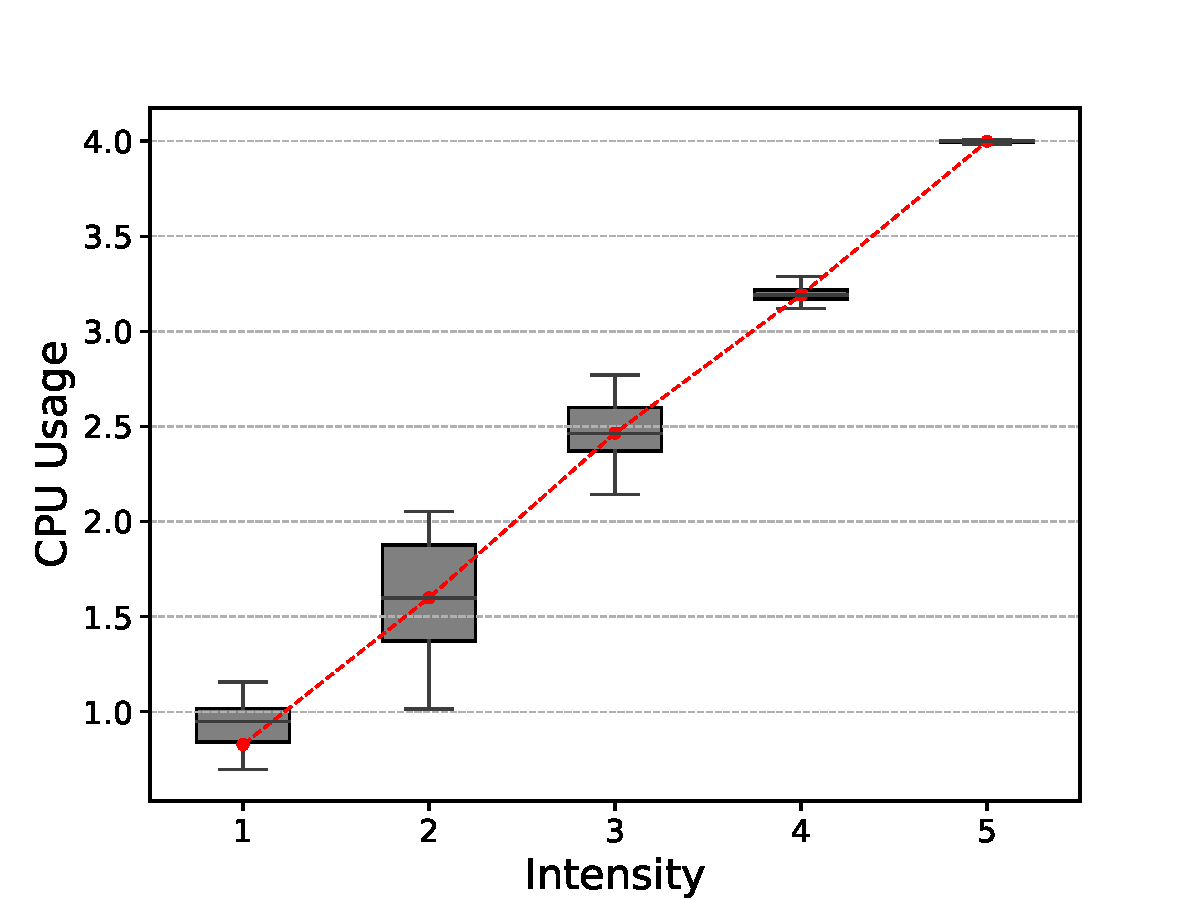
\includegraphics[width=\textwidth]{cpu_interference}
    \caption{cpu干扰效果}
    \label{fig:cpu_interference}
  \end{subfigure}
  \begin{subfigure}[b]{0.45\textwidth}
    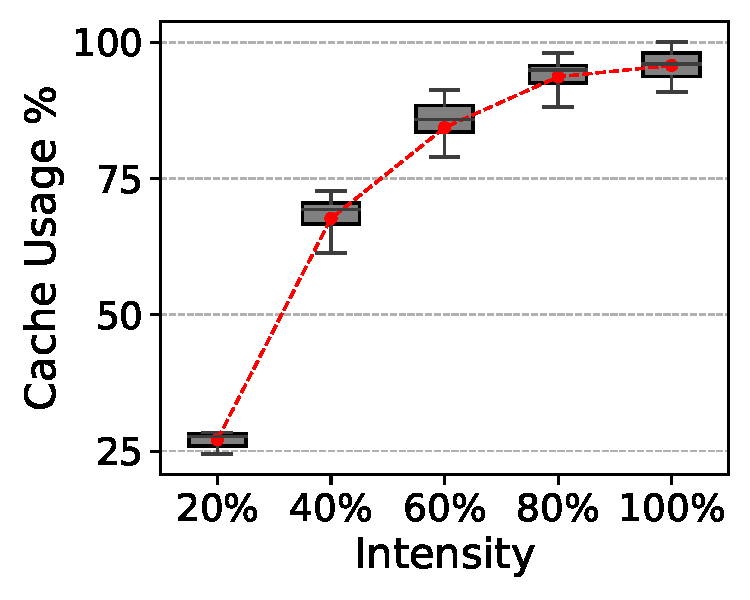
\includegraphics[width=\textwidth]{cache_interference}
    \caption{cache干扰效果}
    \label{fig:cache_interference}
  \end{subfigure}
  \begin{subfigure}[b]{0.45\textwidth}
    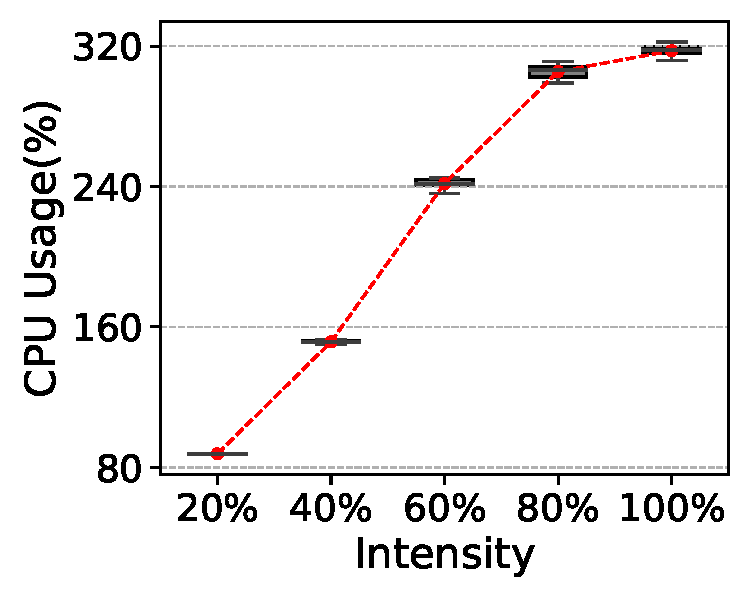
\includegraphics[width=\textwidth]{io_interference}
    \caption{io干扰效果}
    \label{fig:io_interference}
  \end{subfigure}
  \begin{subfigure}[b]{0.45\textwidth}
    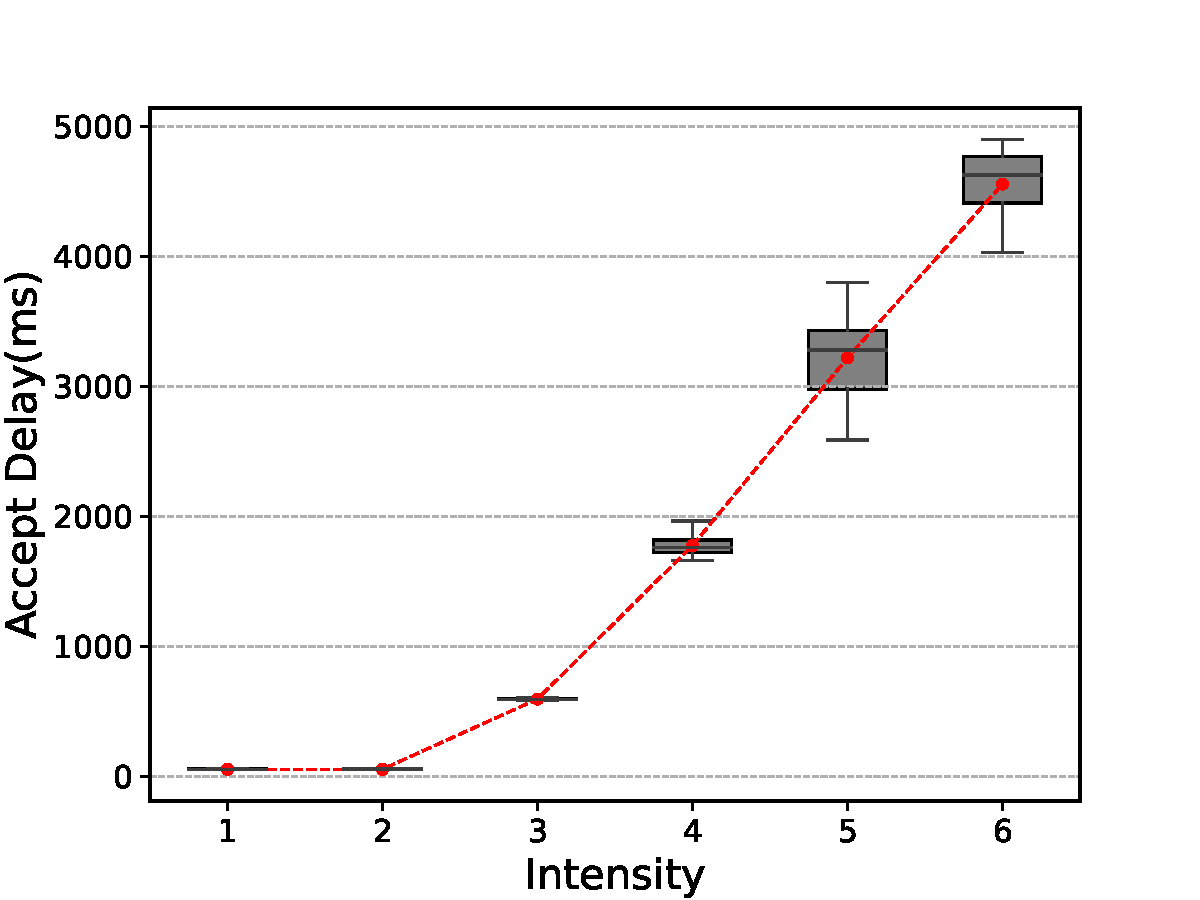
\includegraphics[width=\textwidth]{net_interference}
    \caption{net干扰效果}
    \label{fig:net_interference}
  \end{subfigure}
  \begin{subfigure}[b]{0.45\textwidth}
    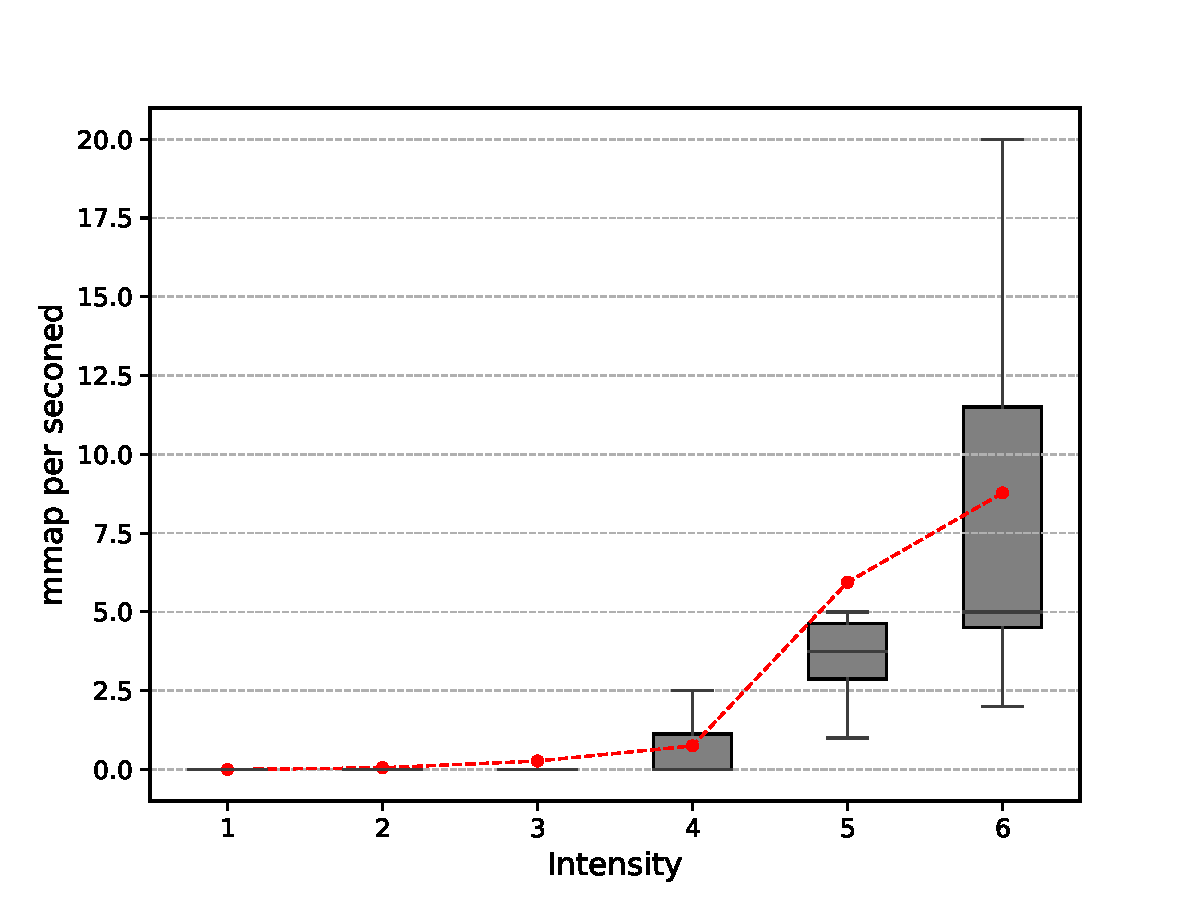
\includegraphics[width=\textwidth]{vm_interference}
    \caption{内存干扰效果}
    \label{fig:vm_interference}
  \end{subfigure}
  \bicaption{\quad 干扰效果分析}{\quad Interference Effects Analysis}
  \label{fig:interference}
\end{figure}

考虑到干扰效果评测结果中,Net干扰实际上使用的是本地回环网络,因此并不能实质性地在网络流量上产生干扰,导致类似于CPU或Cache干扰,因此在后续的
没有采用Net干扰项作为测试项,而是根据典型应用的类型,如是否是网络应用来判断应用的网络敏感性。

\subsection{典型应用资源敏感度分析}

资源敏感度主要分析典型应用与不同配置下的干扰进行混部后的性能劣化情况,其中应用性能使用竖亥Benchmark提供的白盒指标进行评价。白盒指标中既有经过加权计算后的统一评分,也有对于每个应用单独的评价指标,在性能劣化中,主要选择劣化程度与干扰程度较为相关的指标进行分析。

\begin{figure}[H]
    \centering
    \begin{subfigure}[b]{0.45\textwidth}
        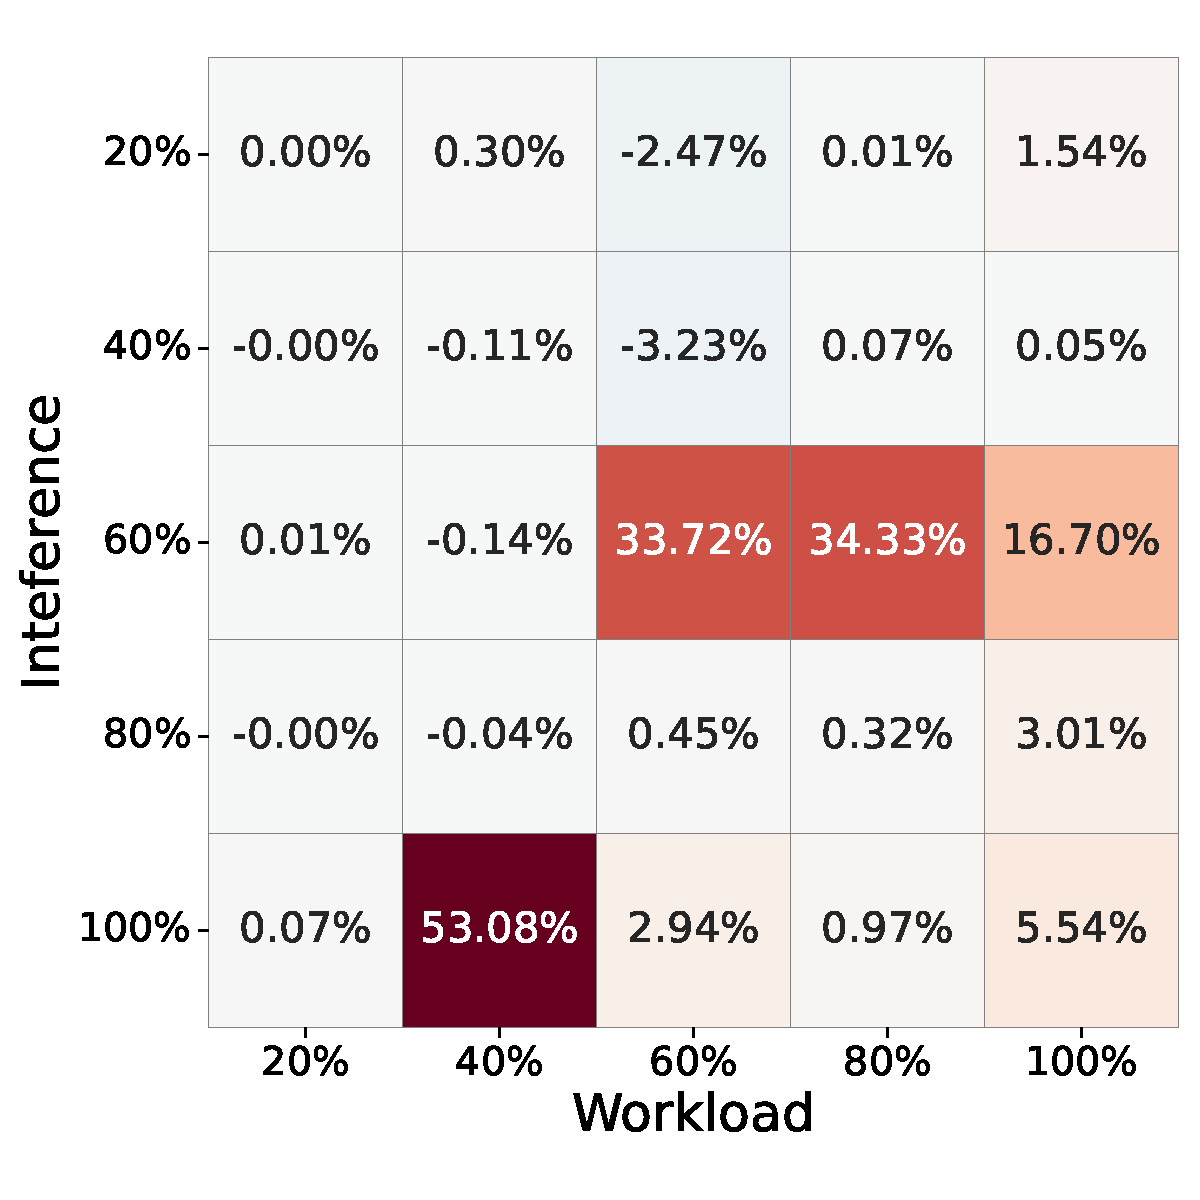
\includegraphics[width=\textwidth]{interfer_cpu}
        \caption{CPU干扰下的性能劣化情况}
        \label{fig:interfer_cpu}
    \end{subfigure}
    \begin{subfigure}[b]{0.45\textwidth}
      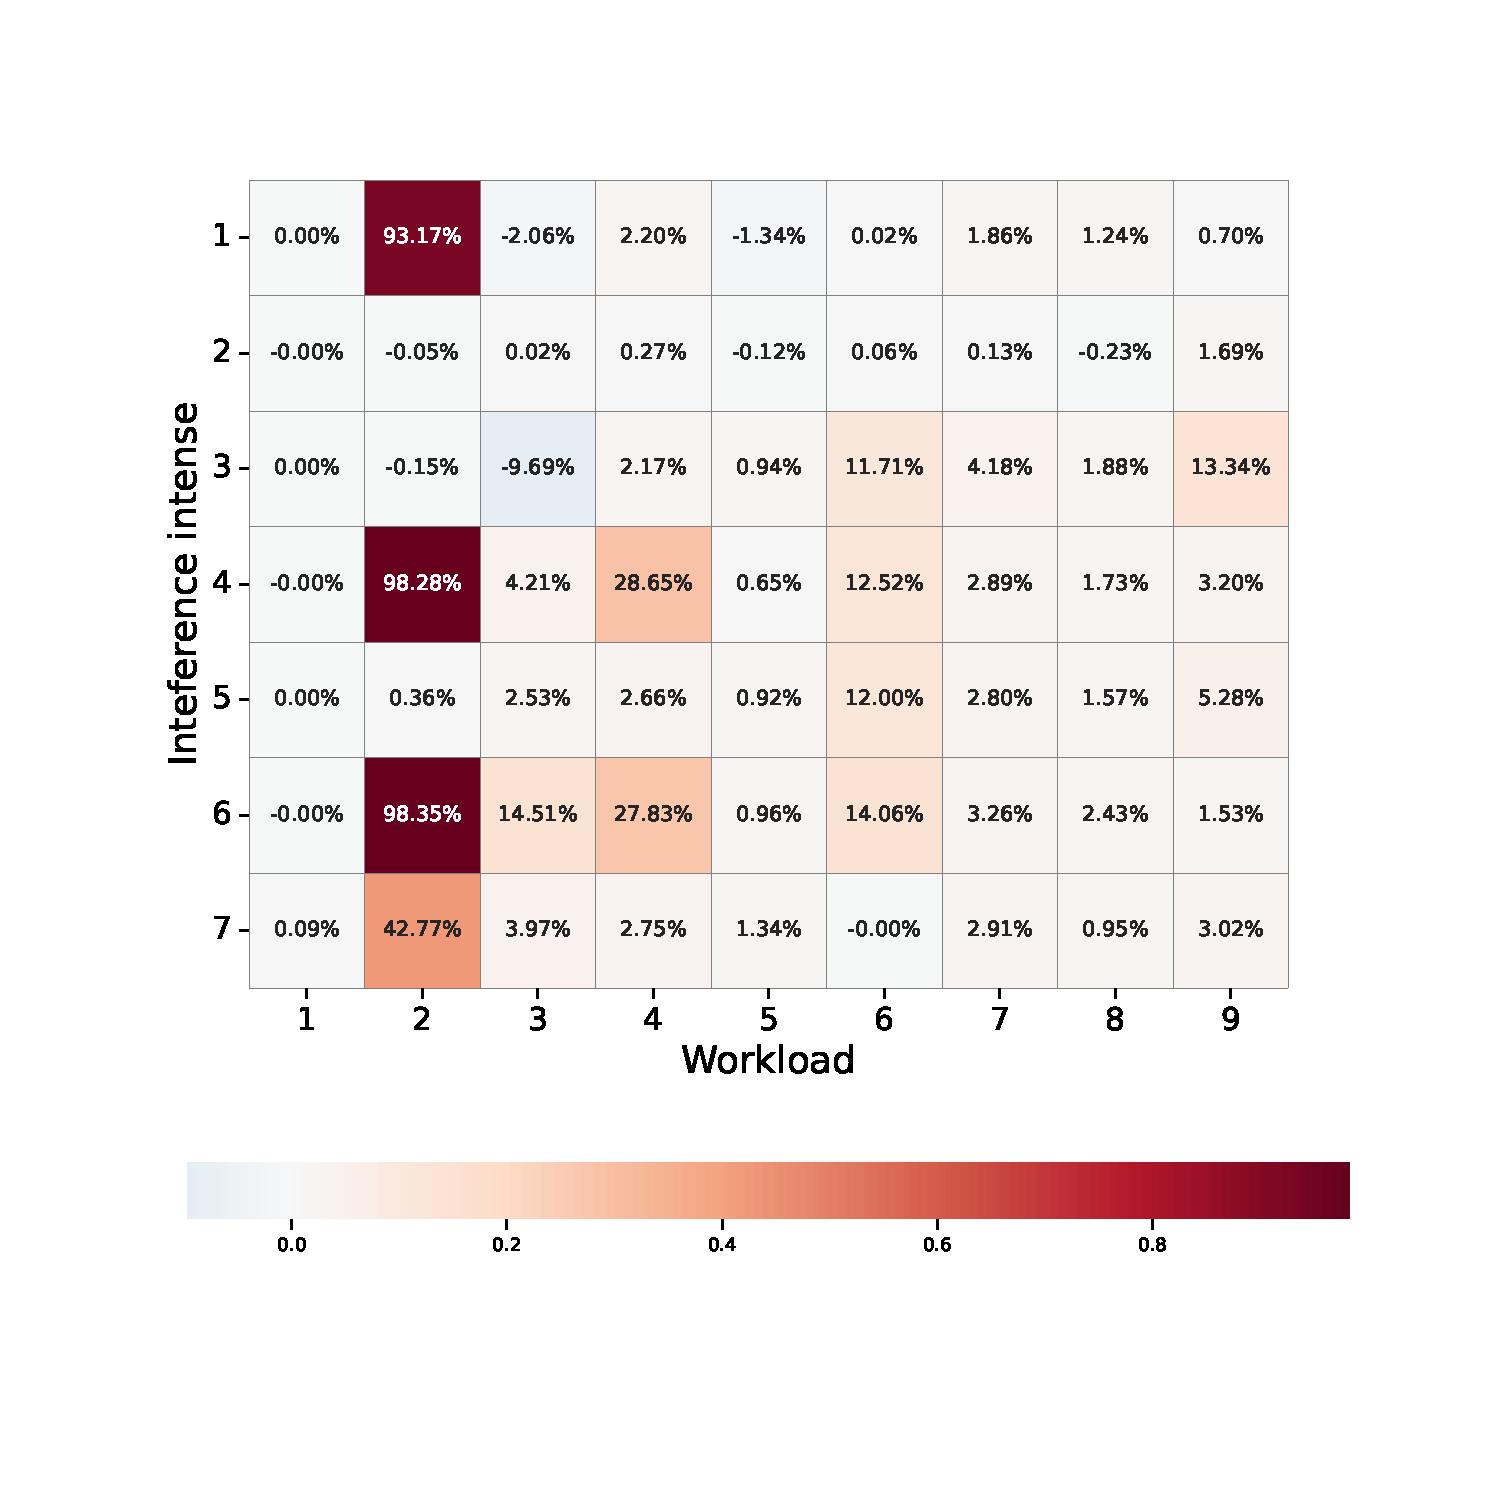
\includegraphics[width=\textwidth]{interfer_cache}
      \caption{Cache干扰下的性能劣化情况}
      \label{fig:interfer_cache}
    \end{subfigure}
    \begin{subfigure}[b]{0.45\textwidth}
        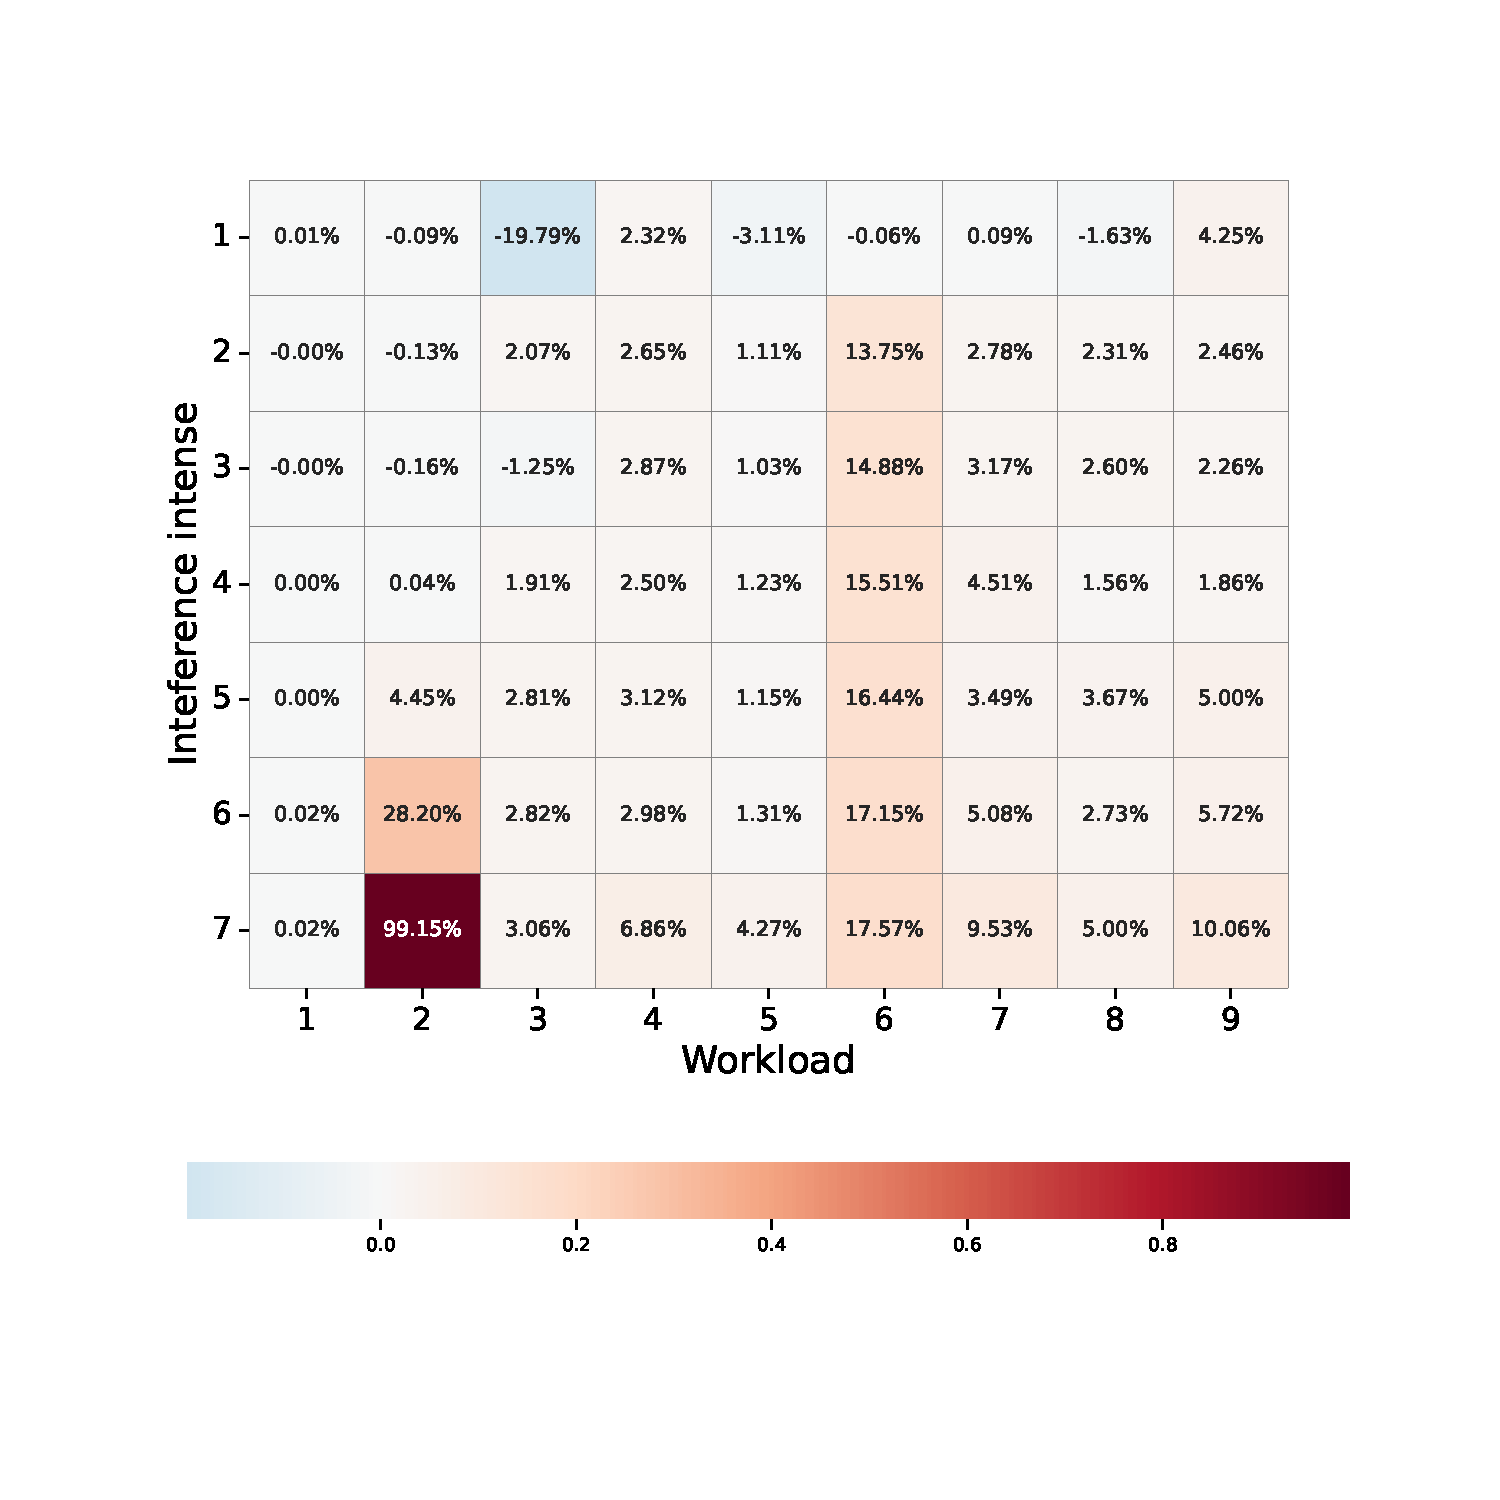
\includegraphics[width=\textwidth]{interfer_io}
        \caption{IO干扰下的性能劣化情况}
        \label{fig:interfer_io}
    \end{subfigure}
    \begin{subfigure}[b]{0.45\textwidth}
        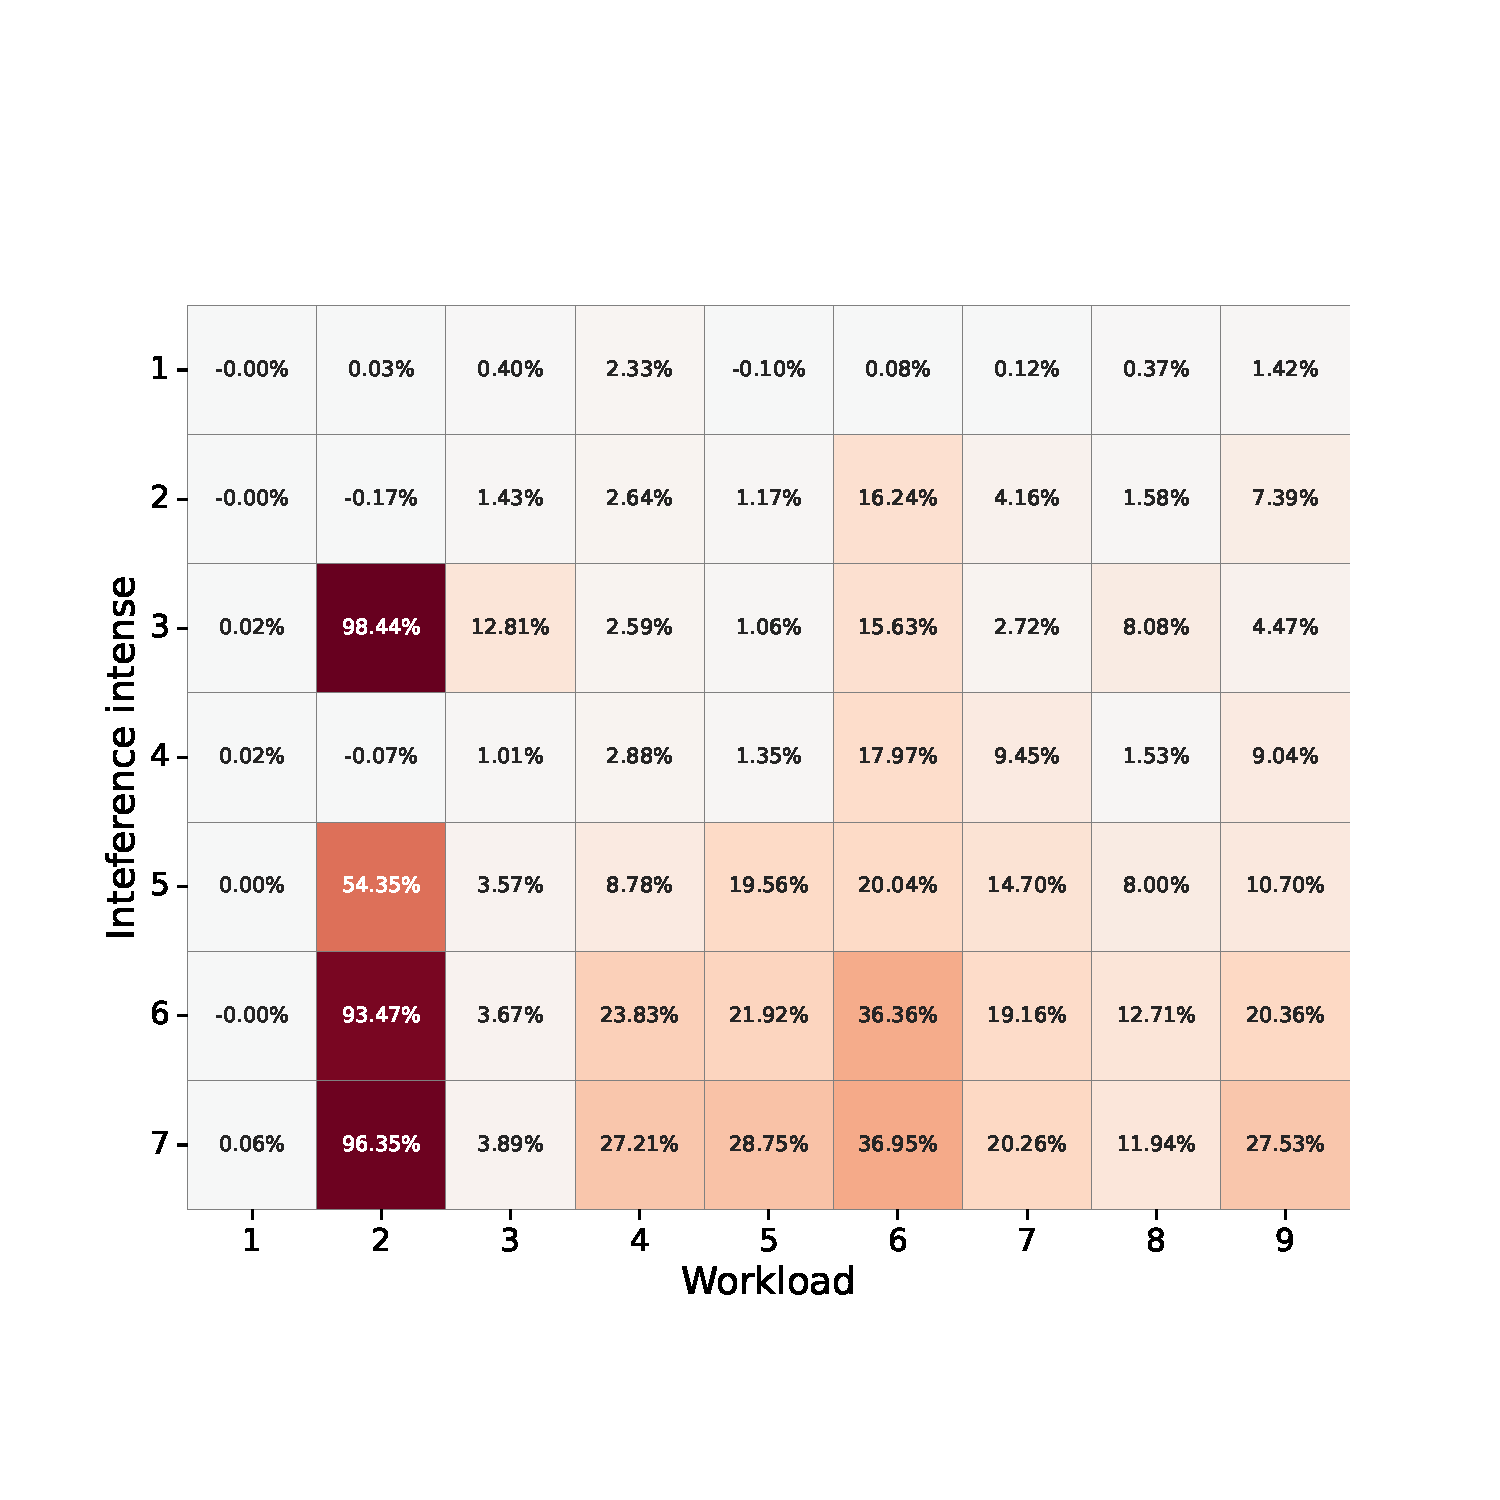
\includegraphics[width=\textwidth]{interfer_mem}
        \caption{Memory干扰下的性能劣化情况}
        \label{fig:interfer_mem}
    \end{subfigure}
\bicaption{\quad Redis干扰敏感度}{\quad Redis interference sensitivity}
\label{fig:redis_interf_sensitivity}
\end{figure}

以Redis为例,使用redis操作延迟作为性能评价指标,计算有无干扰下的指标变化百分比用于描述劣化程度,综合不同干扰及不同负载下的实验结果如图~\ref{fig:redis_interf_sensitivity}所示。

结合其他应用的资源敏感性分析,可在资源的角度对典型应用进行初步划分,主要为如下3类:

\begin{enumerate}
    \item 单纯CPU敏感型:此类应用对于CPU干扰最为敏感,而受其他干扰影响的程度则明显更低。如Memcached,其在受到CPU资源干扰后产生了近50\%的性能劣化,而对于在其他干扰下的劣化程度则在10\%内,同样的情况也在Kafka的实验数据中出现。
    \item CPU与Cache敏感型:此类应用同时受CPU与Cache干扰明显,且通常对CPU干扰更加敏感。如Redis,与Memcached类似,对CPU干扰十分敏感,而同时由于Redis没有开启多线程支持,因此在Cache资源上的竞争能力弱于Memcached,从而更容易受到Cache干扰的影响。Elasticsearch情况则更为复杂,华为云内部Benchmark中提供了不同的白盒指标来表征Elasticsearch的性能,主要分为吞吐量与延迟,以吞吐量作为标准,则Elasticsearch符合CPU敏感型,而以延迟作为标准,则Elasticsearch则更倾向于CPU和Cache敏感型,这种现象在其他典型应用中也有出现,而对于Elasticsearch,其使用场景中更注重吞吐量,因此在本文中将其归类为CPU与Cache敏感型。
    \item 资源不敏感型:此类应用对于所有干扰的敏感度都偏低。实验中Render在各个干扰下都没有出现较为明显的劣化,这主要有两个原因。一方面,在性能指标上,Render应用使用了完成时间作为性能评价指标,而与其他应用的性能指标不同,完成时间这一指标更偏向于整个运行过程的总体性能述而不是单一处理过程的性能,一些突发的性能劣化不会体现在这一指标上,另一方面,内核调度机制上在未作限制时倾向于公平地分配时间,因此干扰程序会因调度的影响向Render出让CPU时间,而当CPU资源总和足够满足Render使用时,性能指标就不会出现较大变化。
\end{enumerate}

\section{混部场景的调度定制实验}

\subsection{响应度优先内核性能}

% redis \ memcached

Control Zone响应度优先配置使用HZ\_1000配置时钟中断,并开启PREEMPT抢占模式。响应度优先内核的优势主要体现在多任务调度场景,因此在实验设计上,选择Redis、Memcached两种CPU敏感型应用来分别与CPU干扰应用混部以构造多任务场景,并使用CloudHypervisor默认提供的内核作为基准进行比较。实验在一个4CPU 512MB内存的Control Zone中进行。

\begin{figure}[H]
    \centering
    \begin{subfigure}[b]{0.49\textwidth}
      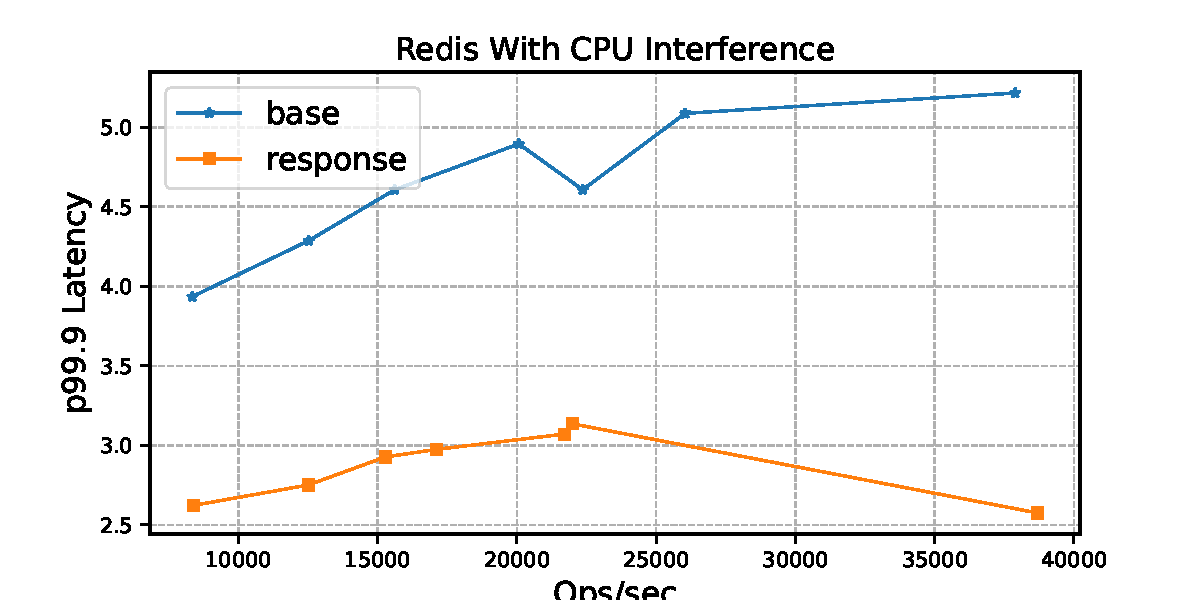
\includegraphics[width=\textwidth]{redis_response}
      \caption{Redis与干扰混部}
      \label{fig:redis_response}
    \end{subfigure}
    \begin{subfigure}[b]{0.49\textwidth}
      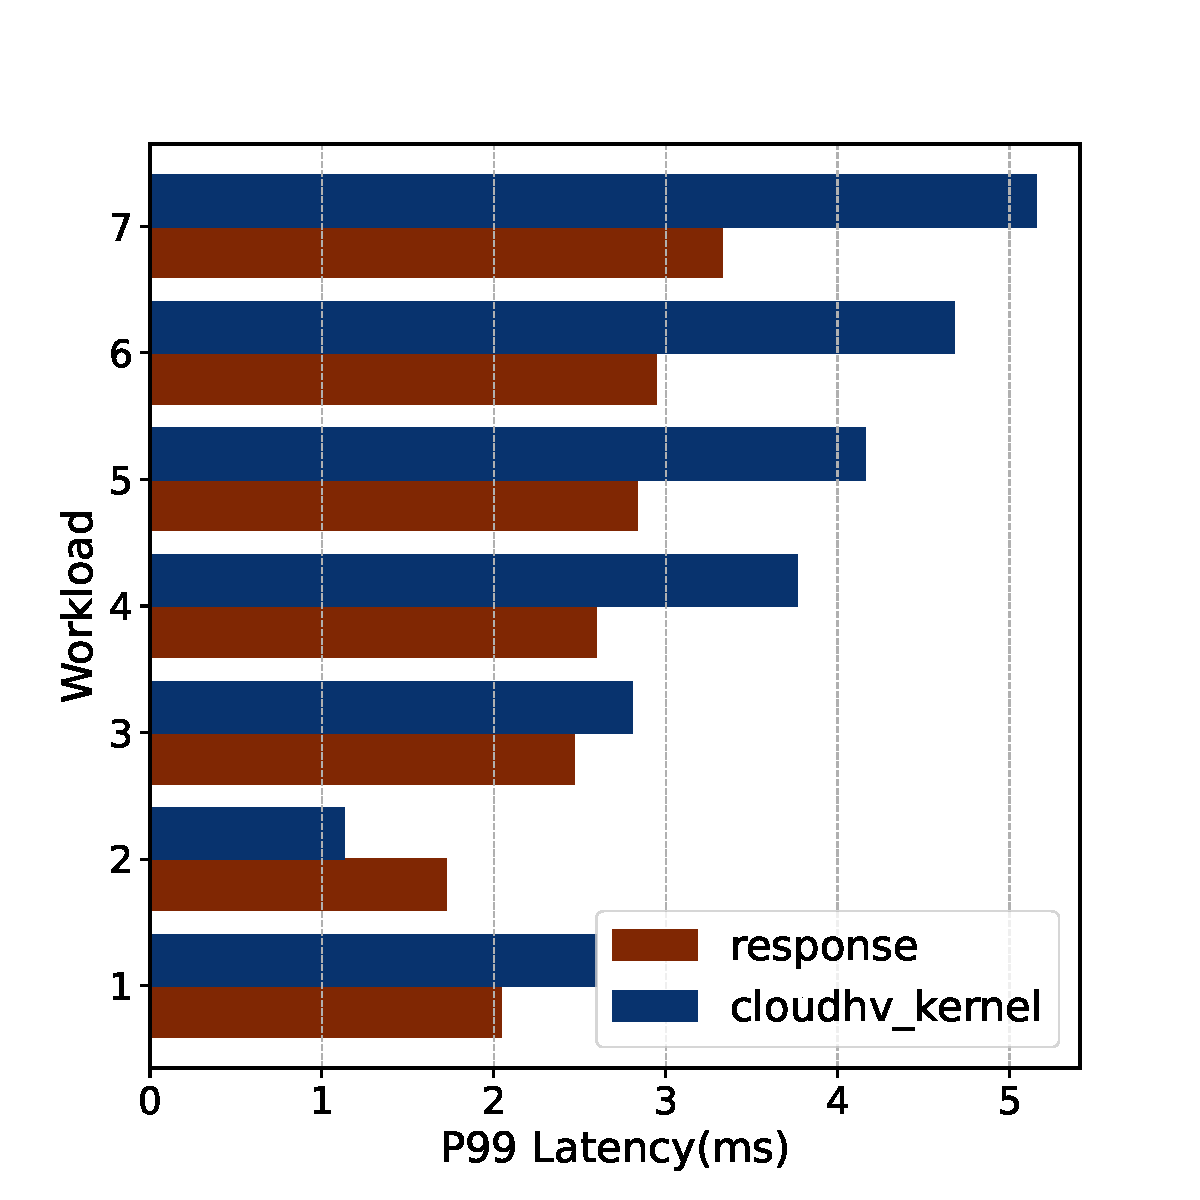
\includegraphics[width=\textwidth]{memcached_response}
      \caption{Memcached与干扰混部}
      \label{fig:memcached_response}
    \end{subfigure}
    \bicaption{\quad 混部场景下的响应度优先内核}{\quad Response Priority Kernel in Mixed Deployment Scenarios}
    \label{fig:lc_response}
\end{figure}

混部实验结果如图~\ref{fig:lc_response}所示,在启用Control Zone响应度优先内核后,无论是Redis还是Memcached,在P99.9延迟上都要优于CloudHypervisor的默认内核,Reponse内核使用了更高的时钟中断频率,因此能够更快地在延时敏感应用与干扰应用中进行切换,同时在PREEMPT抢占模式下,网络中断能够更及时地进行处理,降低请求处理链路的整体延时。

\subsection{吞吐量优先内核性能}

% graph500(time) \ ffmpeg 

Control Zone吞吐量优先配置使用HZ\_100配置时钟中断,并开启PREEMPT\_NONE抢占模式。吞吐量优先内核能够在任务量较少的场景中,让任务保持CPU资源的占用,从而更好地利用局部性,因此实验使用单一任务场景,选择Graph500作为目标应用,并对比其在CloudHypervisor默认内核、Throughput内核以及Response内核下的运行情况。实验在一个4 CPU、512MB内存的Control Zone中进行。

\begin{figure}[H]
    \centering
    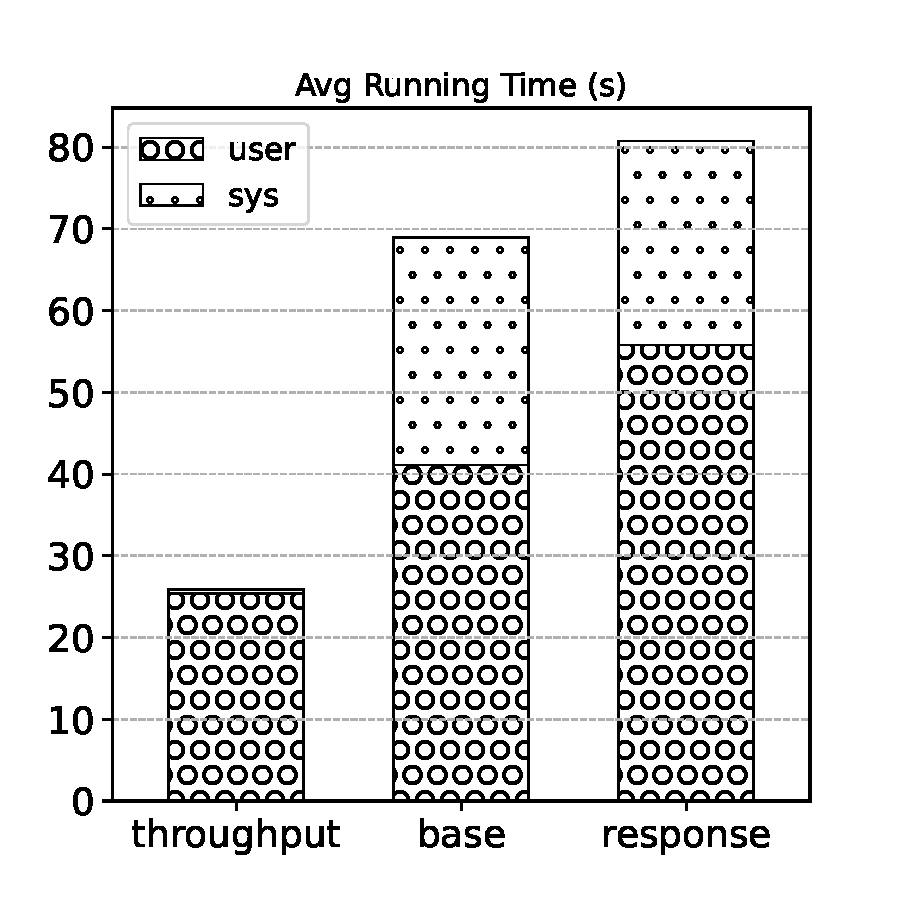
\includegraphics[width=0.5\textwidth]{avg_graph500_runtime}
    \bicaption{\quad 吞吐量优先内核配置优化效果}{\quad Throughput Discrepancy Across Different Configurations} 
    \label{fig:avg_graph500_runtime}
\end{figure}

Graph500主要执行图计算算法,因此执行时间是其重要的性能指标,实验中使用time工具记录任务的执行时间,包括用户态与内核态的执行时间, 具体实验结果如图~\ref{fig:avg_graph500_runtime}所示,其中使用Throughput内核的Control Zone消耗的时间最短,而使用Response内核的Control Zone则消耗的最长的时间,分析执行时间占比,在Throughput内核下,任务运行过程中内核态时间消耗几乎没有,而在Response内核中,内核态时间则占用了较大比例,造成这一结果的主要原因是时钟中断与NO\_HZ配置,越高的时钟中断频率会引发越导致越频繁的陷入内核态,一方面使得内核态时间变得更长,另一方面也会导致局部性的破坏导致任务执行速度的减慢。

\subsection{CPU资源感知策略效果}

% 普通场景
% 硬件场景:SMT

BPF强隔离调度策略能够在混部场景中,为高优先级应用提供更好的性能保障,使得性能接近于无干扰的状态。而为验证强隔离调度策略的效果设计了两个混部场景的实验。场景一中使用4个独立的CPU,2048M内存的Control Zone进行实验,高优先级应用使用Mysql,而低优先级应用使用CPU干扰应用。场景二中则使用2CPU,512M的内存,并特别地使用SMT绑定为虚拟机CPU,同时选用延时敏感的Redis与CPU干扰进行混部。

混部场景一实验结果如图~\ref{fig:mysql_perf}所示,首先能够看出,Linux EEVDF调度器默认下以公平为目标,此时Mysql的性能并不能得到保障,而在降低CPU干扰应用的nice值之后,Mysql的性能虽然有一些提升,但相较于无干扰情况下仍存在较大劣化, 而分析Control Zone CPU使用率能够发现,Mysql在正常运行时并不会占用所有的核心,此时即便与干扰应用存在优先级上的差异,但由于这种优先级并不能跨越CPU调度队列产生效果,因此仍然存在一定程度上的并发,而由于资源竞争的Mysql的性能就会出现劣化。而在启用了BPF调度器之后Mysql性能几乎与没有干扰的情况下一致,首先,尽管优先级机制不能跨越核心产生作用,但在BPF调度器中能够自已强隔离的所里,使得高优先级的Mysql在运行时,低优先级的干扰应用能够自动的让出CPU,从而实现高优先级任务的性能保障。

\begin{figure}[!htbp]
    \centering
    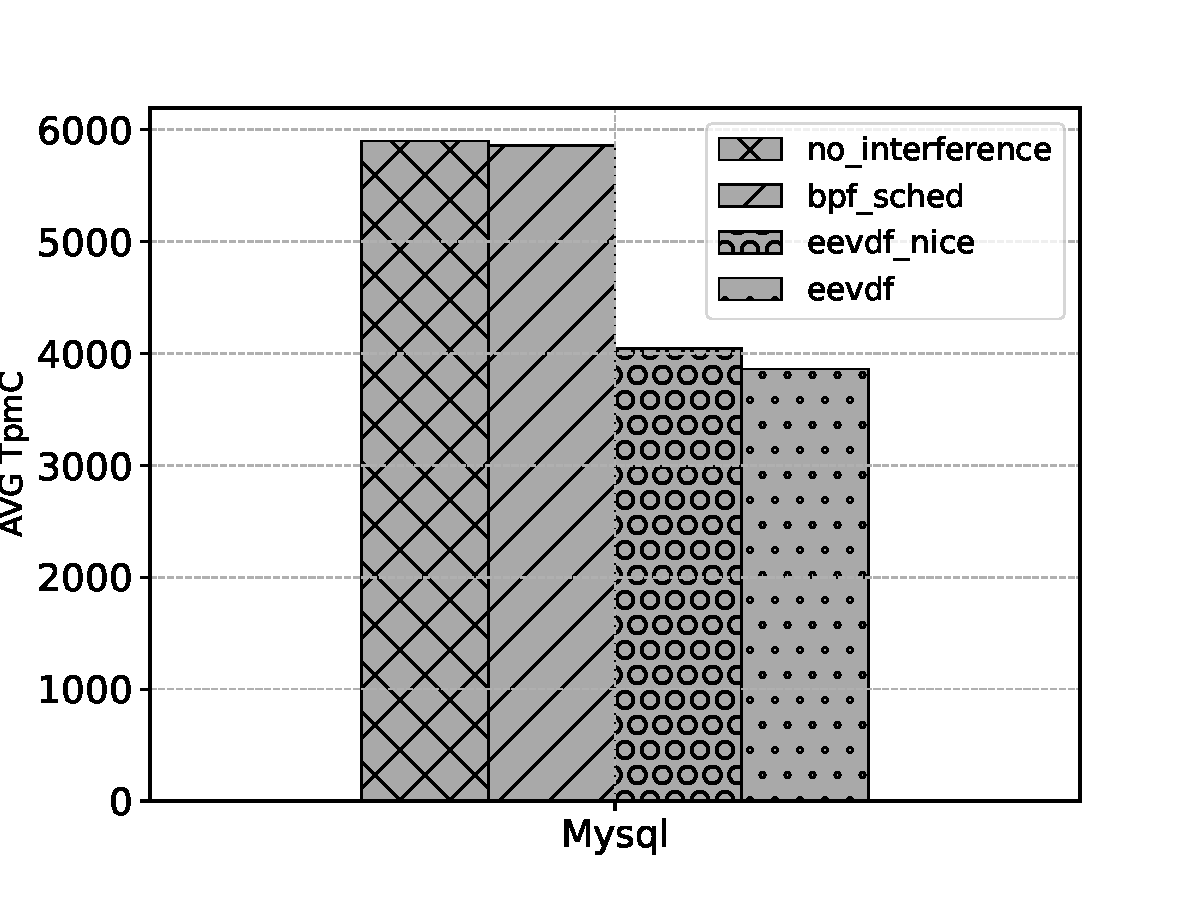
\includegraphics[width=0.6\textwidth]{mysql_perf}
    \bicaption{\quad Mysql与干扰混部}{\quad MySQL with Interference} 
    \label{fig:mysql_perf}
\end{figure}

混部场景二实验结果如图~\ref{fig:redis_smt}所示。SMT下Sibling共享了同一个物理CPU上的片上资源, 因此混部存在更激烈的资源竞争。Elfen\citep{yang2016elfen}通过修改内核与BE应用,使得BE应用能够主动探测Sibling上LC应用并及时出让CPU,从而保障LC应用的性能。这一思路在SMT场景中十分重要,而在BPF CPU感知任务调度策略中,首先,可以在Control Zone的资源声明中标注SMT信息,随后在BPF调度器启动时可以利用此参数,并在调度时考虑Sibling的运行情况。从实验结果中也能够看出,相较于Linux默认调度器,BPF调度器能够在干扰混部的场景中,使得LC应用在低负载时降低79.6\%的延迟,并在高负载时仍有33.7\%的延迟降低效果,这说明BPF Scheduler能够在不同负载下保障LC应用,使其性能接近于无干扰的情况

\begin{figure}[!htbp]
    \centering
    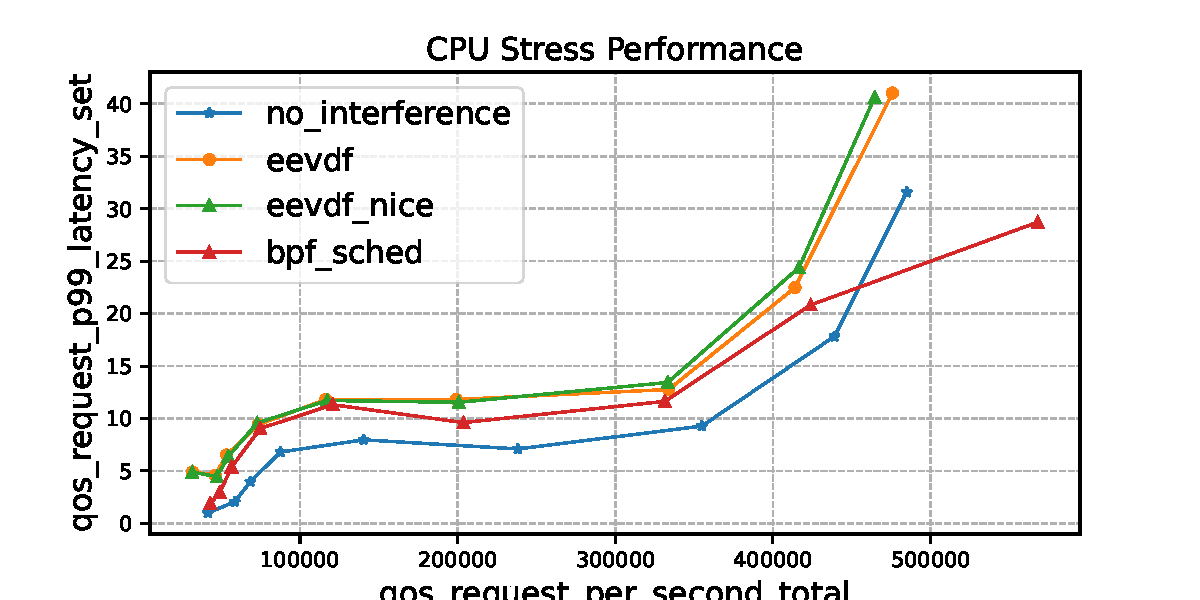
\includegraphics[width=0.6\textwidth]{redis_smt}
    \bicaption{\quad SMT下Redis与干扰混部}{\quad Redis with Interference On SMT} 
    \label{fig:redis_smt}
\end{figure}

\begin{figure}[H]
    \centering
    \begin{subfigure}[b]{0.49\textwidth}
        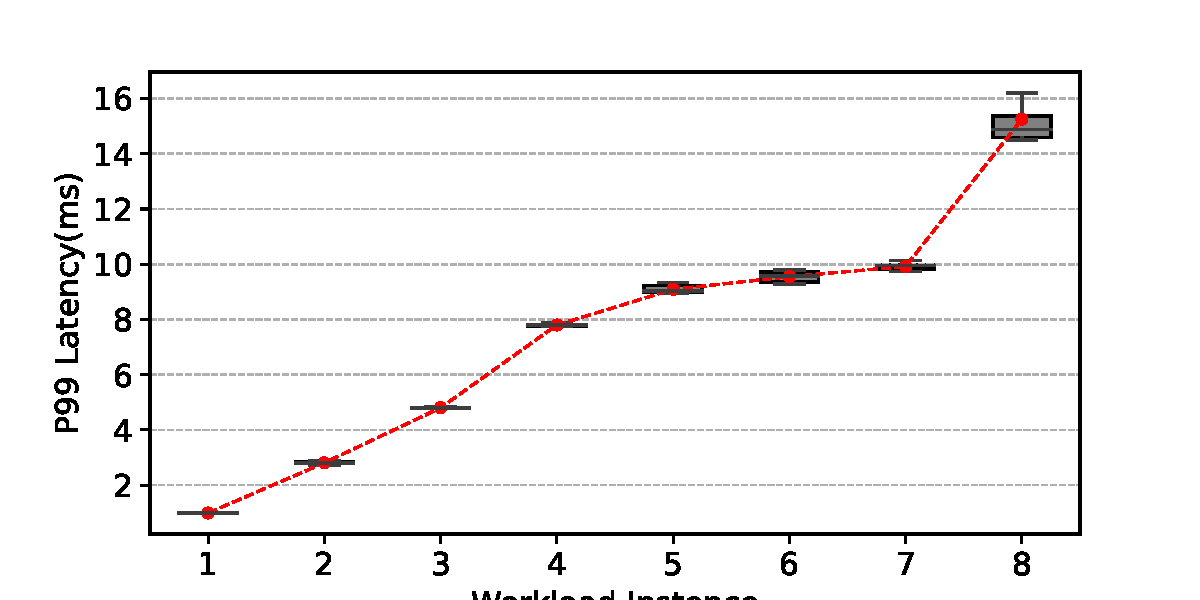
\includegraphics[width=\textwidth]{cpu_aware_box_bpf_sched}
        \caption{无干扰下Redis延迟}
        \label{fig:cpu_aware_box_bpf_sched}
    \end{subfigure}
    \begin{subfigure}[b]{0.49\textwidth}
        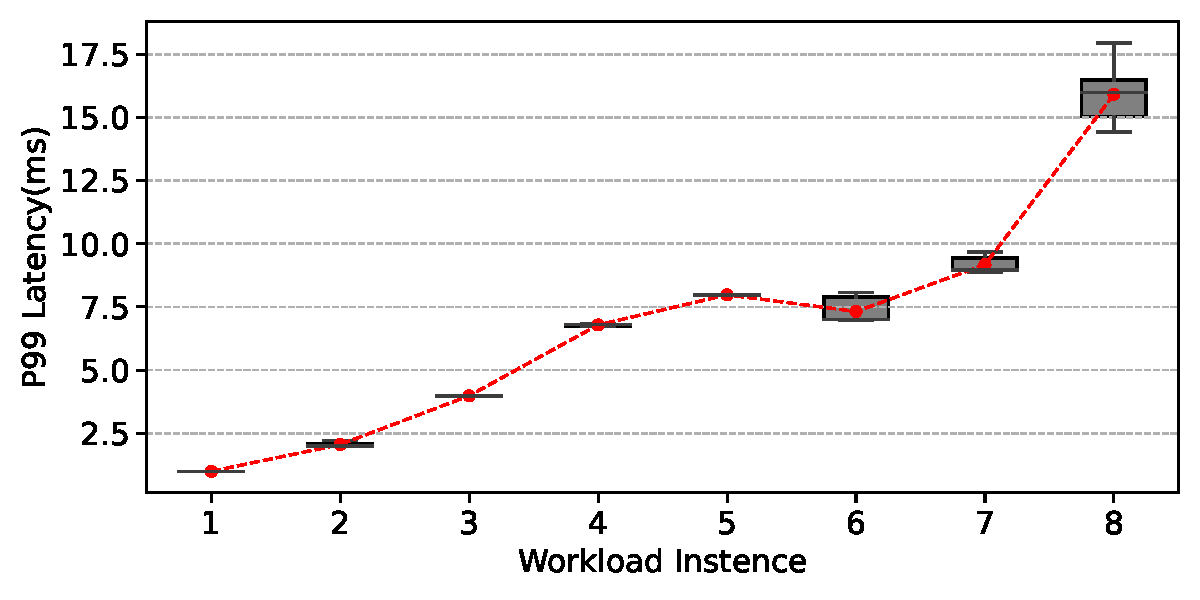
\includegraphics[width=\textwidth]{cpu_aware_box_no_interference}
        \caption{混部场景BPF调度器}
        \label{fig:cpu_aware_box_no_interference}
    \end{subfigure}
    \begin{subfigure}[b]{0.49\textwidth}
        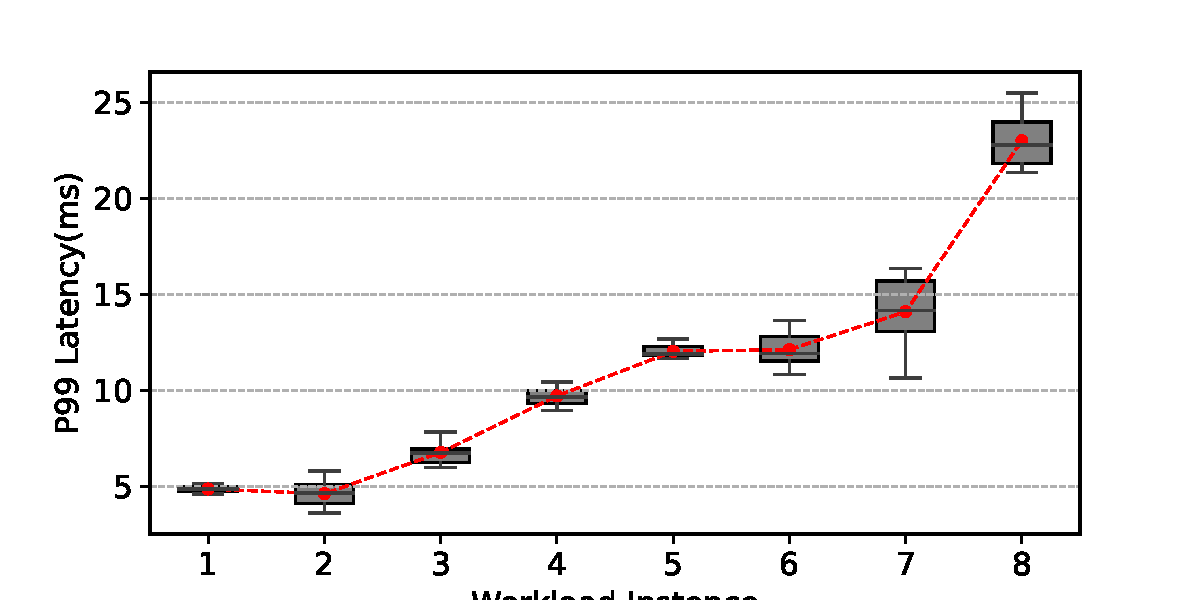
\includegraphics[width=\textwidth]{cpu_aware_box_eevdf}
        \caption{混部场景EEVDF调度器}
        \label{fig:cpu_aware_box_eevdf}
    \end{subfigure}
    \begin{subfigure}[b]{0.49\textwidth}
        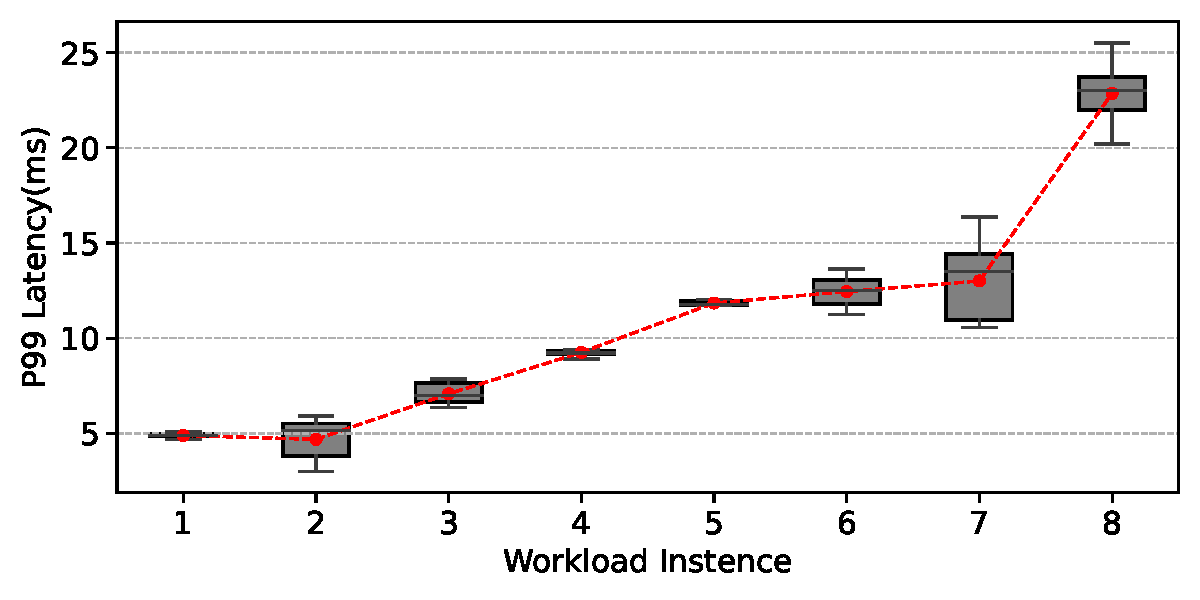
\includegraphics[width=\textwidth]{cpu_aware_box_eevdf_nice}
        \caption{混部场景EEVDF高优先级}
        \label{fig:cpu_aware_box_eevdf_nice}
    \end{subfigure}
\bicaption{\quad LC应用延迟稳定性}{\quad LC Application Latency Stability}
\label{fig:lc_box}
\end{figure}

同时从图~\ref{fig:lc_box}中能够看出,在BPF调度器下,LC应用的延迟稳定性也得到了一定的保障,这一方面是因为BPF调度器中的任务队列隔离机制,使得高优先级的LC应用总是能够被优先调度,另一方面则是因为BPF调度器没有信息墙,能够直接接触并调度任务,这是因为BPF调度器运行在内核中并遵循Core调度框架。

\section{沙箱开销实验}

\subsection{启动开销}

Control Zone的启动开销计算从虚拟化运行时开始到系统引导至init过程的时间,虚拟机使用1CPU与512M内存的基础配置,在虚拟化运行时上,选择CloudHypervisor与Qemu进行对比,而在精简内核上,选择Alpine Virt内核、Control Zone内核,以及CloudHyeprvirsor、Firecracker的默认精简内核,其中Alpine Virt内核为社区提供给云厂商的标准虚拟机内核,启动了大部分Guest优化功能,但同时也保留了对于众多设备的支持,而以轻量为目标的CloudHyeprvirsor、Firecracker也各自提供了默认的精简内核,相较于Alpine Virt内核,去除了大量无意义的驱动,几乎只支持virtio设备,其中CloudHypervisor默认内核还额外使能了PCI子系统,以便于使用SRIOV设备,实验中为了让实验结果更加具备可比性,因此使能了Firecracker内核中的PCI配置。

\begin{figure}[H]
    \centering
    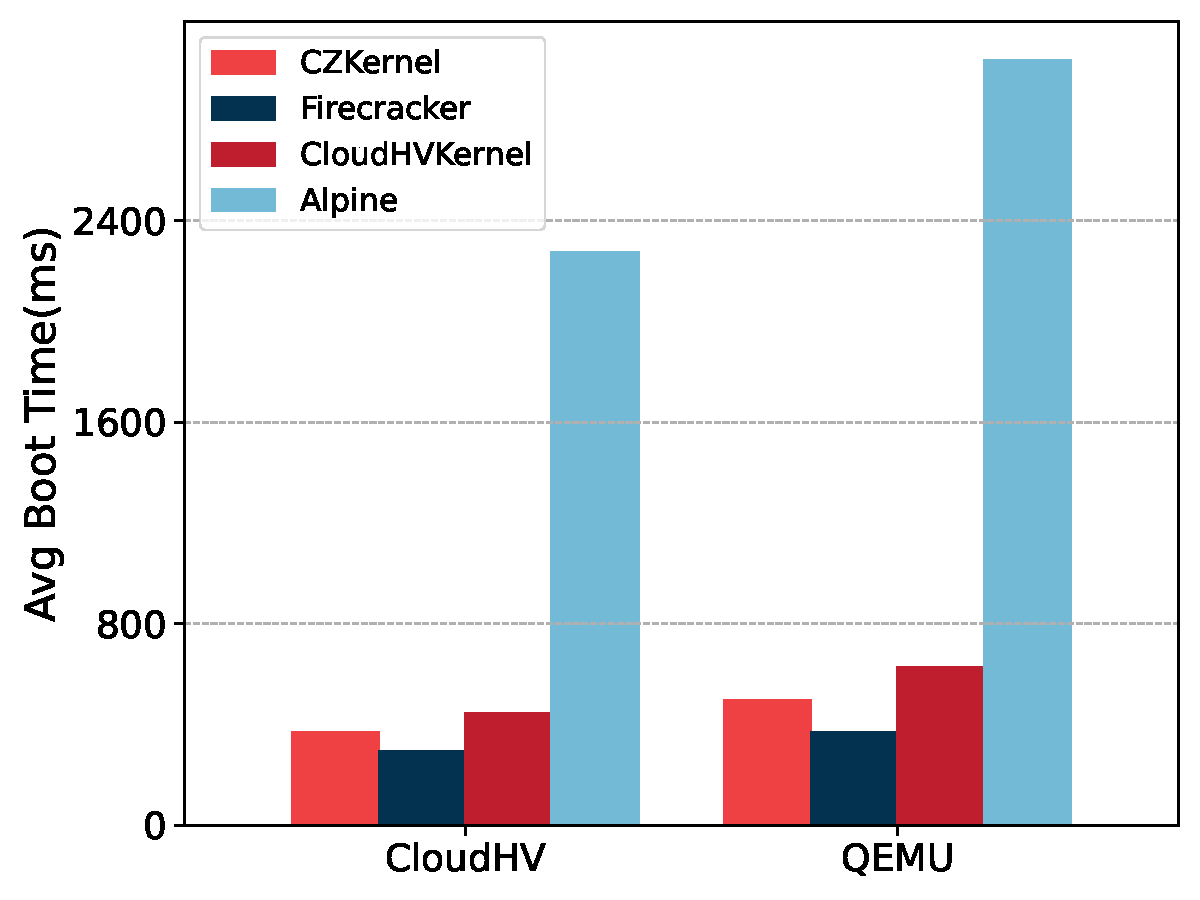
\includegraphics[width=0.55\textwidth]{avg_boot_time}
    \bicaption{\quad 平均启动时间比较}{\quad Comparison of average boot times}
    \label{fig:avg_boot_time}
\end{figure}

实验结果如图~\ref{fig:avg_boot_time}所示,Control Zone内核的平均启动开销相较于Alpine Virt内核最高降低了88.8\%,对比不同的虚拟化运行时的数据发现而其中绝大部分的优化效果升来自于对内核的裁切,Control Zone内核仅支持运行容器、BPF子系统与Sched Ext调度类的最小功能,因此在启动时省去了大量非必要的工作,从而能够做到足够快速。同时还可以发现, 对于Alpine Virt内核而言,使用CloudHypervisor相较于Qemu降低28.9\%的启动时间,而观察两者的启动日志发现,虚拟化运行时所带来的提升主要来自于对于设备的裁切上,CloudHypervisor只需要针对云场景,因此相较于Qemu去除了大量的无关设备模拟,而更精简的设备一方面减少了虚拟化运行时的启动时间,另一方面,Guest内核也不必进行过多的设备探测与初始化,尤其在PCI子系统的初始化上,CloudHypervisor相较于Qemu,PCI子系统的初始化时间平均减少了83.2\%。相同的情况在其他内核上则有所不同,由于精简内核本身支持的设备驱动就十分有限,因此虚拟化运行时在这些内核的优化上主要体现在运行时启动本身上。

\begin{figure}[!htbp]
    \centering
    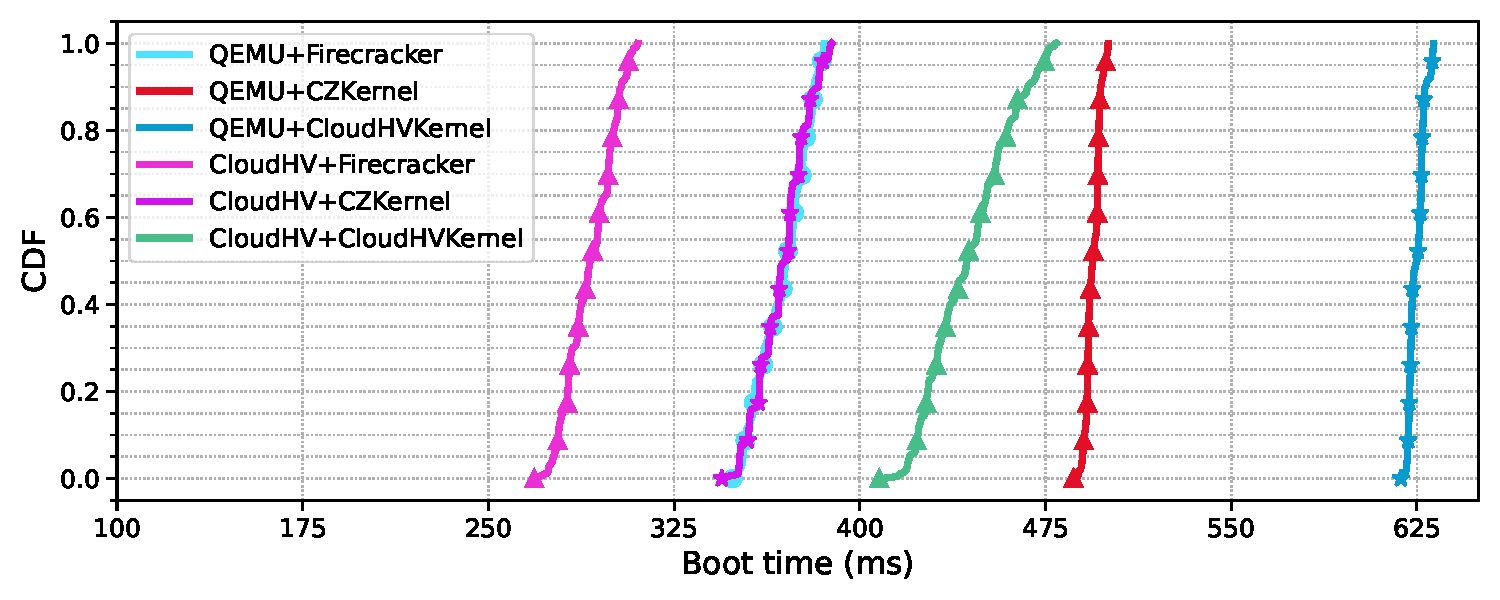
\includegraphics[width=0.8\textwidth]{boot_time_cdf}
    \bicaption{\quad 精简内核的启动时间比较}{\quad Comparison of Kernel Boot Time Optimization} 
    \label{fig:boot_time_cdf}
\end{figure}

在精简内核的对比中,Control Zone内核也存在优势,如图~\ref{fig:boot_time_cdf}所示,使用Qemu时,Control Zone内核相较于CloudHypervisor默认内核在启动时间上减少了20.6\%,对比两者配置差异发现,CloudHypervisor所提供的精简内核虽然去掉了大部的驱动支持,但仍然保留了对嵌套虚拟化的支持而开启了虚拟化子系统,因此会产生额外的开销,而Control Zone内核所支持的容器环境所需要的支持则相对更少。但是相对于Firecra内核,Control Zone内核则在启动开销上并没有优势,即便使用Qemu虚拟化运行时,Firecracker内核也能达到接近使用CloudHypervisor的Control Zone内核的启动速度,比较配置能够发现, Firecracker内核在功能裁切上更加激进,分析两者的启动日志能够发现这开销的差异主要来自于Control Zone内核中所需要的额外功能,如Netfilter子系统等。这些功能在本设计中时必须的,同时考虑场景上的差异,Firecracker实现时希望以承担安全容器的运行时环境,虚拟机的生命周期与运行在其中的容器绑定,而在Control Zone的设计中,任务与Control Zone并非完全耦合,Control Zone更接近与对于隔离环境的声明,在任务需要运行时启动,而在任务运行完毕后仍然会保留,并提供给下一个任务使用,即Control Zone不会频繁地启动,因此这部分开销在设计中是可以接受的。


\section{本章小结}

本章围绕Control Zone沙箱机制设计了一系列实验。。

